\documentclass[11pt]{article}
\usepackage[margin=1in]{geometry}
\usepackage{amsmath,amssymb,amsthm,mathtools}
\usepackage{booktabs,tabularx,array,enumitem,microtype,xcolor}
\usepackage{tikz}
\usetikzlibrary{arrows.meta,positioning}
\usepackage[colorlinks=true,linkcolor=blue!45!black,citecolor=blue!45!black,urlcolor=blue!45!black]{hyperref}
\hypersetup{pdftitle={The shortest binary stabilizer code with three logical qubits and distance six},pdfauthor={Brandon Li}}
\setlength{\emergencystretch}{2em}
\setlength{\belowcaptionskip}{6pt}
\setlist{nosep,leftmargin=*}

\newtheorem{theorem}{Theorem}[section]
\newtheorem{proposition}[theorem]{Proposition}
\newtheorem{lemma}[theorem]{Lemma}
\newtheorem{corollary}[theorem]{Corollary}
\theoremstyle{definition}
\newtheorem{definition}[theorem]{Definition}
\newtheorem{example}[theorem]{Example}
\theoremstyle{remark}
\newtheorem{remark}[theorem]{Remark}

\newcommand{\F}{\mathbb F_2}
\newcommand{\qc}[1]{[\![#1]\!]}
\newcommand{\wt}{\operatorname{wt}}
\newcommand{\cost}{c_R}
\newcommand{\rank}{\operatorname{rank}}
\newcommand{\rad}{\operatorname{rad}}
\newcommand{\im}{\operatorname{im}}
\newcommand{\Ann}{\operatorname{Ann}}
\newcommand{\Span}{\operatorname{span}}
\newcommand{\Hull}{\operatorname{Hull}}
\newcommand{\Aut}{\operatorname{Aut}}
\newcommand{\tr}{\mathsf T}
\newcommand{\pathcode}[1]{{\small\nolinkurl{#1}}}

\title{The shortest binary stabilizer code with three logical qubits and distance six}
\author{Brandon Li\\[0.2em]
\normalsize John L. Miller Great Neck North High School, Great Neck, New York\\
\normalsize\href{mailto:brandon.li.gn@gmail.com}{brandon.li.gn@gmail.com}}
\date{November 2026}

\begin{document}
\maketitle

\begin{abstract}
We show that eighteen is the smallest number of physical qubits needed
for a binary stabilizer code that encodes three logical qubits with
minimum distance six. The main result is the lower bound: no binary
\(\qc{17,3,6}\) stabilizer code exists, pure or degenerate. Integer
certificates for the weight enumerator show that any such code would be
pure and would contain a stabilizer of weight eight. A parity argument
on the remaining nine qubits then leaves five possibilities for the
stabilizers supported on those eight qubits. The rest of the code is
determined by a linear map that must satisfy a commutation equation and
a weight condition, and the kernel of this map splits each possibility
into further cases. We classify all corresponding nine-qubit shortened
codes and run an exhaustive search for such maps, ruling out every case.
For the upper bound, we give fifteen explicit generators of a pure
\(\qc{18,3,6}\) code whose distance can be checked in seconds.
Previously, Grassl's tables left both \(\qc{17,3}\) and \(\qc{18,3}\)
open between distances five and six; our results settle both entries,
giving optimal distances \(5\) and \(6\).
\end{abstract}

\noindent\textbf{Keywords:} quantum error correction; stabilizer codes; additive
codes; optimal codes; nonexistence; shortening; computer-assisted proof.

\noindent\textbf{MSC 2020:} 81P73, 94B65.

%=====================================================================
\section{Introduction}\label{sec:intro}

How many physical qubits does a binary stabilizer code need to encode
three logical qubits, correct arbitrary errors on any two qubits, and
detect arbitrary errors on any five? We show that the answer is
eighteen. Seventeen qubits are not enough, and we exhibit an explicit
code on eighteen.

A stabilizer code \cite{gottesman,crss97,crss} is defined by an abelian
group \(S\) of Pauli operators, called its \emph{stabilizers}. The
\emph{weight} of a Pauli operator is the number of qubits on which it
acts nontrivially. The \emph{centralizer} is the set of all Pauli
operators that commute with every stabilizer in \(S\). The \emph{minimum
distance} \(d\) is the smallest weight of a centralizer operator outside
\(S\)---an undetected operator that alters the
encoded information. An \(\qc{n,k,d}\) code encodes \(k\) logical qubits
in \(n\) physical qubits. A code of distance \(d\) detects arbitrary
errors on up to \(d-1\) qubits and corrects arbitrary errors on up to
\(\lfloor (d-1)/2\rfloor\) qubits \cite{knilllaflamme}. Distance six is
therefore the threshold in our question.

Let \(d_{\max}(n,k)\) be the largest minimum distance of a binary
stabilizer code on \(n\) physical qubits encoding \(k\) logical qubits.
For small \(n\) and \(k\), Grassl's tables \cite{grassl} record both the
best known achievable distance and the best known upper bound. Whenever
these two numbers differ, the entry is open: either a better code
exists, or the upper bound can be lowered.

The entries \((n,k)=(17,3)\) and \((18,3)\) are two such cases. For
both, the tables list a distance-five code obtained by extending a
\(\qc{15,3,5}\) code by two or three qubits. Meanwhile, the linear
programming bound with the shadow identities
\cite{shorlaflamme,rains98,ashikhmin,rains} still permits distance six.
Before this work, \(5\leq d_{\max}(17,3)\leq6\) and
\(5\leq d_{\max}(18,3)\leq6\), and the shortest code in the tables
encoding three qubits with distance six used twenty qubits. Our main
results rule out distance six at length seventeen and construct a code
of distance six at length eighteen.

\begin{theorem}\label{thm:main}
There is no binary stabilizer code with parameters \(\qc{17,3,d}\) for
any \(d\geq6\). Hence \(d_{\max}(17,3)=5\).
\end{theorem}

\begin{theorem}\label{thm:code}
The fifteen Pauli operators in Table~\ref{tab:gens} generate a pure
\(\qc{18,3,6}\) stabilizer code. Hence \(d_{\max}(18,3)=6\).
\end{theorem}

\begin{corollary}\label{cor:length}
A binary \(\qc{n,3,d}\) stabilizer code with \(d\geq6\) exists if and
only if \(n\geq18\).
\end{corollary}

A stabilizer code is \emph{pure} if it contains no nontrivial
stabilizers of weight below its distance \(d\), and \emph{degenerate}
otherwise. Theorem~\ref{thm:main} covers both pure and degenerate codes:
rather than assuming purity, we prove that any \(\qc{17,3,6}\) code must
be pure. Throughout, we consider only stabilizer (additive) codes;
nonadditive codes are not addressed.

\subsection*{The idea of the proof}

We prove Theorem~\ref{thm:main} by contradiction. Suppose a
\(\qc{17,3,6}\) code \(S\) exists. The proof proceeds in three steps,
summarized in Figure~\ref{fig:flow}.

\emph{Step 1: purity and a weight-eight stabilizer.} A distance-six code
can still contain stabilizers of weight below six. Fixing a hypothetical
stabilizer of weight below six, we count all stabilizers by their weight
on its support (the qubits where it acts nontrivially) and outside its
support. Linear identities relate these counts to the centralizer and to
a parity-shifted coset called the \emph{shadow}, yielding linear systems
with no nonnegative solution. Each infeasibility is certified by an
explicit list of integer multipliers, which can be checked in exact
arithmetic. This shows that \(S\) is pure, that it contains a stabilizer
\(p\) of weight eight, and that it has at most two stabilizers of weight
six or seven.

\emph{Step 2: split the code across the weight-eight stabilizer.} Let
\(T\) be the support of \(p\). Keeping only centralizer operators that
act trivially on \(T\) and dropping the coordinates in \(T\) leaves a
\emph{shortened code} \(C\) on the remaining nine qubits. A parity
argument shows that a nine-qubit additive code (a binary linear subspace
of Pauli operators) of minimum weight six has binary dimension at most
six. Consequently, the stabilizers supported on \(T\) form a subspace
\(R\) of dimension one or two, and up to equivalence there are five
possibilities for \(R\). The shortened code \(C\) belongs to one of
\(32{,}865\) or \(56\) equivalence classes, which we classify and
certify to be complete. An extension criterion
(Theorem~\ref{thm:extension}) then encodes the rest of the code as a
linear map \(M\) from local operators on \(T\) to cosets of \(C\),
subject to a commutation equation and a weight inequality. The kernel of
\(M\) consists of logical operators supported on \(T\); its dimension
and the hull of \(C\) (its intersection with its orthogonal complement)
split each type into a small number of cases.

\emph{Step 3: search every case.} For each type, equivalence class, and
kernel case, an exhaustive computer search looks for such a map \(M\)
and finds none.

\begin{figure}[htbp]
\centering
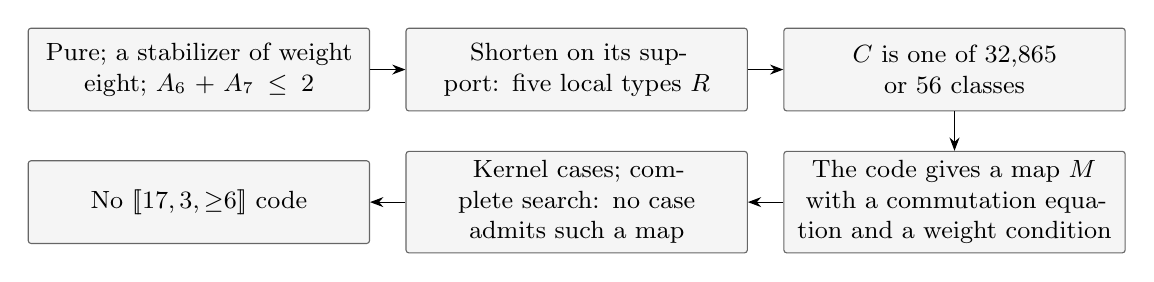
\begin{tikzpicture}[>=Stealth,
 box/.style={draw=black!60,fill=black!4,rounded corners=1pt,
 text width=4.1cm,minimum height=1.05cm,align=center,font=\small},
 node distance=0.5cm and 0.45cm]
\node[box] (a) {Pure; a stabilizer of weight eight; \(A_6+A_7\leq2\)};
\node[box,right=of a] (b) {Shorten on its support: five local types \(R\)};
\node[box,right=of b] (c) {\(C\) is one of \(32{,}865\) or \(56\) classes};
\node[box,below=of c] (d) {The code gives a map \(M\) with a commutation equation and a weight condition};
\node[box,left=of d] (e) {Kernel cases; complete search: no case admits such a map};
\node[box,left=of e] (f) {No \(\qc{17,3,{\geq}6}\) code};
\draw[->] (a)--(b); \draw[->] (b)--(c); \draw[->] (c)--(d); \draw[->] (d)--(e); \draw[->] (e)--(f);
\end{tikzpicture}
\caption{Structure of the proof of Theorem~\ref{thm:main}.}
\label{fig:flow}
\end{figure}

Checking Theorem~\ref{thm:code} requires no search. The fifteen
generators are printed in full, and verifying distance six is a finite
computation: the Pauli operators of weight at most two have pairwise
distinct commutation patterns (\emph{syndromes}) with the generators, no
operator of weight three shares a syndrome with any of them, and an
explicit centralizer operator outside the stabilizer has weight six.
Corollary~\ref{cor:length} follows immediately from the two theorems,
because any code can be extended by one qubit without lowering its
distance.

Several recent methods address \((n,k,d)=(17,3,6)\) without settling it.
The semidefinite programming bounds of Angl\`es Munn\'e, Nemec, and
Huber \cite{mnh} apply to all quantum codes, and Angl\`es Munn\'e and
Huber \cite{sdp} made them rigorous via rational certificates. For
\((n,d)=(17,6)\), their Table~1 gives \(4\leq K\leq8\) for the
code-space dimension, leaving \(K=2^3=8\) open. Lai \cite{lai} develops
refined weight-enumerator and structural tests, which do not decide this
case either \cite[Section~\mbox{VII-D}]{lai}.

Our proof uses neither method. It combines weight-enumerator
certificates with a structural reduction and a finite search, in the spirit of the proof by
Bierbrauer et al.\ \cite{bierbrauer} that no \(\qc{13,5,4}\) code
exists; related geometric methods for purity and local structure appear
in \cite{geometry}. Weight-enumerator arguments have also settled the
existence of several small codes of maximal distance \cite{hgs,hg}. For
the neighboring entry \((n,k)=(14,3)\), Singh \cite{singh} announced the
nonexistence of \(\qc{14,3,5}\) codes, including degenerate ones, and
Lai \cite[Section~VII-C1]{lai} also gives a proof. Our classifications
build on the classification of small additive codes of distance five by
Grassl, Krotov, Sok, and Sol\'e \cite{dodeca}. The same method shows
that no \(\qc{16,5,5}\) code exists; that proof, together with a
\(\qc{17,5,5}\) code, appears separately \cite{li16}.

Cohen, Encheva, and Litsyn \cite{cel} reported an \(\qc{18,3,6}\) code
constructed from binary codes. In Remark~\ref{rem:cel} we explain why
the matrix printed there does not yield such a code; Grassl's tables
list a lower bound of five for \((18,3)\).

The paper is organized as follows. Section~\ref{sec:prelim} introduces
the binary Pauli notation. Section~\ref{sec:forced} proves Step~1 and
derives the five local types. Section~\ref{sec:extension} establishes
the extension criterion together with the kernel and hull identities
used in Steps~2 and~3. Section~\ref{sec:classification} proves that the
classifications are complete, and Section~\ref{sec:search} describes the
search for extension maps. Sections~\ref{sec:rank-two}
and~\ref{sec:rank-one} exclude the rank-two and rank-one types.
Section~\ref{sec:proof} assembles the proof of Theorem~\ref{thm:main}
and summarizes the computational checks. Finally, Section~\ref{sec:code}
presents the \(\qc{18,3,6}\) code, proves Theorem~\ref{thm:code}, and
deduces Corollary~\ref{cor:length}.

%=====================================================================
\section{Preliminaries}\label{sec:prelim}

We represent \(n\)-qubit Pauli operators, ignoring global phases, as
binary vectors of length \(2n\) \cite{crss}. All vector spaces are over
the two-element field \(\F=\{0,1\}\), and we set
\[
 V_n=\F^{2n}=\{(x\mid z):x,z\in\F^n\},\qquad
 \langle(x\mid z),(x'\mid z')\rangle=x\cdot z'+z\cdot x'.
\]
On each qubit, the bit pairs \((0,0),(1,0),(0,1),(1,1)\) represent the
Pauli letters \(I,X,Z,Y\). Vector addition in \(V_n\) corresponds to
multiplying Pauli operators up to phase. The \emph{symplectic inner
product} \(\langle u,v\rangle\in\F\) is \(0\) when \(u\) and \(v\)
commute, and \(1\) when they anticommute. A subspace of \(V_n\) is
\emph{isotropic} if every pair of vectors in it has symplectic product
\(0\), meaning that all its Pauli operators commute. We refer to vectors
in this space as \emph{words}. The \emph{support} of a word is the set
of coordinates where its letter is not \(I\), and its \emph{weight}
\(\wt(x\mid z)=|\{i:(x_i,z_i)\ne(0,0)\}|\) is the size of its support.
A \emph{\(Z\)-only} word has letters \(I\) and \(Z\), so its
\(X\)-component vanishes.

The weight-parity function \(\varepsilon(v)=\wt(v)\bmod2\) satisfies
\begin{equation}\label{eq:polar}
 \varepsilon(u+v)=\varepsilon(u)+\varepsilon(v)+\langle u,v\rangle,
\end{equation}
as one checks coordinate by coordinate: any two distinct nonidentity
Pauli letters anticommute, and their sum is the third nonidentity
letter. Thus \(\varepsilon\) is a quadratic form whose associated
bilinear form is the symplectic inner product. In particular, a subspace
on which every word has even weight is isotropic, and \(\varepsilon\) is
linear on every isotropic subspace.

A binary \(\qc{n,k}\) stabilizer code is an isotropic subspace
\(S\leq V_n\) of dimension \(n-k\), with Pauli phases omitted. Its
\emph{centralizer} is its symplectic orthogonal complement
\(D=S^\perp\), which consists of all Pauli operators commuting with
every stabilizer and has dimension \(n+k\). For \(k>0\), its minimum
distance is
\[
 d(S)=\min\{\wt(w):w\in S^\perp\setminus S\}.
\]
Elements of \(S^\perp\setminus S\) act nontrivially on the encoded
information, whereas stabilizers act trivially, so low-weight
stabilizers are permitted. A code is \emph{pure to distance \(d\)} if
every nonzero word of its centralizer has weight at least \(d\). For a
code of distance at least \(d\), this simply means that no nonzero
stabilizer has weight below \(d\). We write \(A_j\) for the number of
stabilizers of weight \(j\); the sequence of these counts is the
\emph{weight enumerator}.

An \emph{additive code} of length \(\ell\) is any \(\F\)-linear
subspace \(C\leq V_\ell\); it need not be isotropic. Its minimum
distance \(d(C)\) is the smallest weight of a nonzero codeword, with
\(d(\{0\})=+\infty\). The notation \((\ell,2^c,d)_4\) denotes an
additive code of length \(\ell\), binary dimension \(c\), and minimum
distance \(d\) over the four-letter Pauli alphabet;
\((\ell,2^c,{\geq}d)_4\) denotes minimum distance at least \(d\). Two
additive codes are \emph{physically equivalent} if one is carried onto
the other by a permutation of coordinates together with independent
permutations of \(X,Y,Z\) at each coordinate. Because
\(\mathrm{GL}(2,2)\) acts as all permutations of the three nonidentity
letters and equals \(\mathrm{Sp}(2,2)\), these relabelings preserve both
weight and commutation. On stabilizer codes, they are precisely qubit
permutations combined with single-qubit Clifford operations, and they
preserve \(\qc{n,k,d}\) and all counts \(A_j\). In particular, any
stabilizer of weight \(w\) can be mapped to
\(Z^w=Z\otimes\cdots\otimes Z\) on its support.

Partition the coordinates into a set \(T\) of size \(m\) and its
complement of size \(f=n-m\). Write \(V_n=V_T\oplus W\), where \(V_T\)
consists of the words acting as \(I\) outside \(T\) and \(W=V_{T^c}\)
consists of those acting as \(I\) on \(T\); we identify \(W\) with
\(V_f\). Let \(\pi_T\) and \(\pi_W\) be the two coordinate projections.
We call a word on \(T\) a \emph{prefix} and a word on its complement a
\emph{suffix}. For a subspace \(R\leq V_T\), write \(R_T^\perp\) for its
orthogonal complement inside \(V_T\). Intersecting a code with
\(W\)---keeping only the words that act as \(I\) on \(T\) and dropping
the coordinates in \(T\)---produces its \emph{shortened code} on
\(T^c\). Given a subspace \(C\leq W\), a \emph{coset} of \(C\) is a
translate \(w+C\); the cosets form the quotient space \(W/C\).

The following lemma records the dimension and minimum distance of a
shortened centralizer.

\begin{lemma}[Shortening]\label{lem:shorten}
Let \(S\) be an \(\qc{n,k}\) code, let \(T\) be a set of \(m\)
coordinates, and put \(R=S\cap V_T\) and \(r=\dim R\). Then
\(\pi_T(S^\perp)=R_T^\perp\), and \(C=S^\perp\cap W\) has binary
dimension
\begin{equation}\label{eq:dimC}
 \dim C=(n+k)-(2m-r).
\end{equation}
If \(S\) is pure to distance \(t\), then \(C\) is an additive
\((n-m,2^{n+k-2m+r},{\geq}t)_4\) code.
\end{lemma}
\begin{proof}
A word \(u\in V_T\) is orthogonal to \(\pi_T(S^\perp)\) if and only if
it is orthogonal to \(S^\perp\), that is, \(u\in S\cap V_T=R\). Hence
\(\pi_T(S^\perp)=R_T^\perp\), which has dimension \(2m-r\). Because the
kernel of \(\pi_T\) on \(S^\perp\) is \(C\), the rank--nullity theorem
gives \eqref{eq:dimC}. Every nonzero word of \(C\) is also a nonzero
word of \(S^\perp\), so purity implies that it has weight at least
\(t\).
\end{proof}

Table~\ref{tab:notation} collects the main symbols used in
Sections~\ref{sec:extension}--\ref{sec:rank-one}.

\begin{table}[htbp]
\centering\small
\caption{Main notation.}\label{tab:notation}
\begin{tabularx}{\linewidth}{@{}lX@{}}\toprule
Symbol&Meaning\\\midrule
\(n,k,d\)&Physical qubits, encoded qubits, and target distance\\
\(S,D=S^\perp,A_j\)&Stabilizer, centralizer, and stabilizer weight counts\\
\(T,m,f\)&Selected support, its size, and complementary size \(n-m\)\\
\(R,r\)&Stabilizer supported on \(T\), and its dimension\\
\(C,P=C^\perp\)&Shortened centralizer, and its dual on the complement\\
\(E,a,b\)&Local quotient \(R_T^\perp/R\), its dimension, and \(\dim P\)\\
\(M,\tau,\Gamma\)&Extension map, its symplectic adjoint, and the Gram matrix on \(P\)\\
\(K,q,t\)&Kernel of \(M\), its dimension, and its restricted form rank\\
\(N,h\)&Kernel of \(\tau\), and hull dimension \(\dim(C\cap C^\perp)\)\\
\(H\)&Local centralizer \(S^\perp\cap V_T\)\\
\(\sigma,c_R,\delta\)&Syndrome map, local coset minimum weight, and complementary coset minimum weight\\
\(\varepsilon,\mathcal{K}_j^\ell\)&Weight-parity function and quaternary Krawtchouk polynomial\\
\(\mu\)&Half the local quotient dimension\\\bottomrule
\end{tabularx}
\end{table}

%=====================================================================
\section{Purity, a weight-eight stabilizer, and the local types}\label{sec:forced}

Assume that \(S\leq V_{17}\) is a \(\qc{17,3,d\geq6}\)
stabilizer code, so \(\dim S=14\), \(|S|=2^{14}\), and \(\dim S^\perp=20\).
Recall that the counts \(A_j\) include all elements of the group,
including products of basis generators.
This section proves that \(S\) is pure, that it contains a word of
weight eight, and that the stabilizer supported on such a word has one
of five types.

\subsection{Exact weight-enumerator certificates}\label{sec:certificates}

Weight-enumerator equations constrain the number of words of each weight
without specifying the code itself. The MacWilliams identities
\cite{shorlaflamme,rains98} express the weight counts of the centralizer
in terms of those of the stabilizer, and the shadow identities
\cite{rains} supply further nonnegative counts. A \emph{certificate} is
an integer linear combination of these necessary relations that yields a
contradiction under a stated case assumption, and it can be checked in
integer arithmetic alone.

The ordinary weight enumerator records only total weight. A \emph{split
weight enumerator} \cite{macwilliams,laiashikhmin} also records how many
nonidentity letters fall in each block of a coordinate partition. We
need this when a prescribed stabilizer word or subgroup is supported on
one block. The formulas below apply the MacWilliams and shadow
identities independently to each block.

Partition the physical coordinates into blocks of sizes
\(n_1,\ldots,n_s\). Let \(A^{\rm split}_{\mathbf i}\) count stabilizer
words with split weight \(\mathbf i=(i_1,\ldots,i_s)\). Set
\(B=|S|=2^{n-k}\), and define the quaternary Krawtchouk polynomial
\[
 \mathcal{K}_j^{\ell}(w)=\sum_{u=\max(0,j-\ell+w)}^{\min(j,w)}
          (-1)^u3^{j-u}\binom wu\binom{\ell-w}{j-u}.
\]
Character orthogonality gives the centralizer count
\[
 |\{v\in S^\perp:\operatorname{splitwt}(v)=\mathbf j\}|
 =B^{-1}\mathcal T_{\mathbf j},\quad
 \mathcal T_{\mathbf j}=\sum_{\mathbf i}
       \left(\prod_\ell \mathcal{K}_{j_\ell}^{n_\ell}(i_\ell)\right)A^{\rm split}_{\mathbf i}.
\]
This formula rests on the character identity
\[
 \mathbf 1_{v\in S^\perp}=B^{-1}\sum_{s\in S}(-1)^{\langle v,s\rangle}.
\]
The sum equals \(B\) when every word of \(S\) commutes with \(v\), and
zero otherwise. Summing over all words of a fixed split weight produces
the products of Krawtchouk polynomials above, showing that the
transformed coefficients count actual centralizer words.
On an isotropic stabilizer, the weight-parity function is linear by
\eqref{eq:polar}. The affine set
\[
 \mathcal A=\{v:\langle v,s\rangle=\wt(s)\bmod2
                          \text{ for every }s\in S\}
\]
is a nonempty coset of \(S^\perp\), because every linear functional on
\(S\) extends to the ambient space; this coset is the \emph{shadow} of
\(S\) \cite{rains}. Character orthogonality gives its split weight
counts as \(B^{-1}\widehat{\mathcal T}_{\mathbf j}\), where
\[
 \widehat{\mathcal T}_{\mathbf j}=\sum_{\mathbf i}(-1)^{\sum i_\ell}
       \left(\prod_\ell \mathcal{K}_{j_\ell}^{n_\ell}(i_\ell)\right)A^{\rm split}_{\mathbf i}.
\]
Both transforms are nonnegative. Centralizer inclusion and the distance
bound give
\[
 \mathcal T_{\mathbf j}\geq BA^{\rm split}_{\mathbf j},\qquad
 \mathcal T_{\mathbf j}=BA^{\rm split}_{\mathbf j}\quad(1\leq\textstyle\sum j_\ell<d).
\]
These relations hold without assuming purity.

If a prescribed isotropic subgroup \(R_i\) is supported on block \(i\),
we list every coset of \(R_i\) in \(R_i^\perp\). Its \emph{weight
pattern} \(p=(p_0,\ldots,p_{n_i})\) counts the words of each physical
weight in that coset. Let \(y\geq0\) count stabilizer cosets grouped by
their block patterns and suffix weight. Each split count is then the
corresponding linear combination of products of the \(p_j\)'s. On a
block with no prescribed subgroup, we may instead use the split counts
themselves as variables. Every actual stabilizer containing the
prescribed subgroups gives such nonnegative variables, because it is
closed under their addition. The model does not need to reconstruct a
linear code from an arbitrary feasible point; only necessity is used.

The row families are:
\begin{center}\small
\begin{tabularx}{\linewidth}{@{}lX@{}}\toprule
Row&Definition\\\midrule
Unit&\(A^{\rm split}_{\mathbf0}=1\).\\
Total&\(\sum A^{\rm split}_{\mathbf i}=B\).\\
Low distance&\(\mathcal T_{\mathbf j}-BA^{\rm split}_{\mathbf j}=0\), \(1\leq\sum j_\ell<d\).\\
Inclusion&\(BA^{\rm split}_{\mathbf j}-\mathcal T_{\mathbf j}\leq0\).\\
Centralizer&\(-\mathcal T_{\mathbf j}\leq0\).\\
Shadow&\(-\widehat{\mathcal T}_{\mathbf j}\leq0\).\\
Weight assumptions&\(\sum_{\sum i_\ell=w}A^{\rm split}_{\mathbf i}=A_w\), or its explicitly assumed lower bound.\\
Coset relations&A specified linear relation valid separately on every physical pattern.\\\bottomrule
\end{tabularx}
\end{center}
The checker verifies each coset relation against the regenerated
patterns, and no property of a later shortened code is inserted into
these reductions. Allowing the variables to take nonnegative real values
only enlarges the feasible set, so infeasibility of the resulting linear
system still excludes every actual code. Integrality is used separately
in the parity and counting steps below.

Write the system as \(Ez=b\), \(Gz\leq g\), \(z\geq0\). A certificate
consists of arbitrary integer equality multipliers \(\nu\) and
nonnegative integer inequality multipliers \(\lambda\) such that
\[
 c=\nu E+\lambda G\geq0,\qquad \nu b+\lambda g<0.
\]
We verify \(c\geq0\) coordinate by coordinate: since every variable in
\(z\) is nonnegative, this forces \(cz\geq0\). Equality rows may take
multipliers of either sign, whereas inequality rows require nonnegative
multipliers so that their directions are preserved. Any feasible \(z\)
would therefore satisfy \(0\leq cz\leq\nu b+\lambda g<0\), a
contradiction. The checker tests every coefficient column and the
negative right-hand side in exact integer arithmetic. Although the
multipliers may be found by numerical optimization, the certificate is
checked using integer arithmetic alone.

\subsection{Purity and the weight-eight word}

\begin{proposition}[Exact enumerator consequences]\label{prop:17-enumerator}
The hypothetical code is pure to distance six, contains a stabilizer word
of weight eight, and satisfies
\begin{equation}\label{eq:light-budget}
 A_6+A_7\leq2.
\end{equation}
\end{proposition}
\begin{proof}
The split-coset integer certificates for stabilizer weights one through
five exclude all five possibilities without assuming purity. For a
proposed word of weight \(w\), local Clifford operations normalize it
to \(Z^w\); the linear system uses the coset-pattern columns of
\(\langle Z^w\rangle\) on its support, together with the low-distance
equations through weight five. Hence \(A_1=\cdots=A_5=0\), which implies
purity because the logical distance is at least six. With these zeros
imposed, the ordinary weight-enumerator system together with \(A_8=0\)
has an exact infeasibility certificate with negative right-hand side
\(-3{,}932{,}160\). The six certificates are:
\begin{center}\small
\begin{tabular}{@{}lrr@{}}\toprule
Case&Columns&Negative right-hand side\\\midrule
Weight 1&17&\(-786{,}432\)\\
Weight 2&48&\(-5{,}324{,}800\)\\
Weight 3&45&\(-442{,}368\)\\
Weight 4&84&\(-81{,}920\)\\
Weight 5&78&\(-114{,}688\)\\
Pure, \(A_8=0\)&18&\(-3{,}932{,}160\)\\\bottomrule
\end{tabular}
\end{center}
Here ``Columns'' means the number of nonnegative variables in the
expanded system.

For the last assertion, write \(\mathcal{K}_j(w)=\mathcal{K}_j^{17}(w)\)
and \(B=2^{14}\). The low-weight equations are
\(\sum_w \mathcal{K}_j(w)A_w-BA_j=0\) for \(1\leq j\leq5\), and the
shadow inequalities are \(-\sum_w(-1)^w\mathcal{K}_j(w)A_w\leq0\).
Combine the unit row \(A_0=1\) with multiplier \(-1{,}835{,}008\),
the total row with multiplier 116, the five low-weight rows with
\((60,25,11,3,1)\), the five purity rows \(A_j=0\) (\(1\leq j\leq5\))
with \((-851968,-278528,-507904,-147456,-180224)\), and the shadow rows
\(j=0,\ldots,4\) with \((88,32,18,4,2)\). This yields
\(32768(A_6+A_7)\leq65536\), and dividing by 32768 proves
\eqref{eq:light-budget}.
\end{proof}

\subsection{A nine-coordinate dimension bound}

The following bound on additive codes is what makes the weight-eight
word useful. Its proof relies on a weight-parity property that is not
captured by the first few nonnegative MacWilliams coefficients alone.

\begin{lemma}[A nine-coordinate dimension bound]\label{lem:nine-bound}
An additive code on nine coordinates with minimum distance at least six has
binary dimension at most six.
\end{lemma}
\begin{proof}
Any code of larger dimension contains a seven-dimensional subcode, so
suppose \(|C|=128\) with nonzero weight counts \(A_6,A_7,A_8,A_9\)
summing to 127. Nonnegativity of the first three dual MacWilliams
coefficients gives
\[
 A_7+2A_8+3A_9\leq102,\qquad
 A_8+3A_9\geq75,\qquad
 3(A_7+A_8)-4A_9\geq17.
\]
The first two inequalities imply \(A_7\leq3A_9-48\), hence \(A_9\geq16\),
as well as \(A_7+A_8\leq27\). The third then forces \(A_9\leq16\).
Equality throughout forces \((A_6,A_7,A_8,A_9)=(84,0,27,16)\).

On a binary additive code, weight parity is a quadratic form whose
failure to be additive is the symplectic product in \eqref{eq:polar}.
For a quadratic form \(\varepsilon\) on a \(c\)-dimensional binary space
\(U\), define its \emph{Gauss sum} by
\[
 G(\varepsilon)=\sum_{v\in U}(-1)^{\varepsilon(v)}.
\]
For weight parity, this is the number of even-weight words minus the
number of odd-weight words. If the associated bilinear form has rank
\(2\rho\), then \(G(\varepsilon)\) is zero or \(\pm2^{c-\rho}\). Indeed,
squaring the sum and substituting \(y=x+z\) gives
\[
 G(\varepsilon)^2=2^c\sum_{z\in\rad(U)}(-1)^{\varepsilon(z)}.
\]
Because the restriction of
\(\varepsilon\) to the radical is linear, the last sum vanishes if that
restriction is nonzero, and otherwise equals \(|\rad(U)|=2^{c-2\rho}\).
This proves the asserted possibilities. By contrast, the forced weight
distribution would give Gauss sum \(128-2\cdot16=96\). Since \(c=7\) and
\(0\leq\rho\leq3\), the possible nonzero absolute values are
\(128,64,32,16\), none of which is 96. This contradiction proves the
bound.
\end{proof}

\subsection{The five local types}\label{sec:types}

Choose a weight-eight stabilizer word \(p\), set
\(T=\operatorname{supp}p\), and normalize \(p=Z^8\). Let \(R=S\cap V_T\)
and \(r=\dim R\). By Lemma~\ref{lem:shorten}, the shortened centralizer
has length nine and dimension \(4+r\); by purity, its minimum distance
is at least six. Lemma~\ref{lem:nine-bound} therefore gives
\(1\leq r\leq2\). The rest of the argument applies to every choice of
the weight-eight word \(p\).

If \(r=1\), then \(R=\langle Z^8\rangle\). If \(r=2\), choose
\(\zeta\in R\setminus\langle p\rangle\), and let \(\alpha\) be the
number of coordinates where \(\zeta\) has an \(X\)-component. It is even
by commutation. Because both \(\zeta\) and \(\zeta+p\) have weight at
least six, we have \(8+\alpha\geq12\), so \(\alpha\in\{4,6,8\}\). Local
Clifford operations fixing \(Z\) replace \(Y\) by \(X\) on those coordinates. On
the remaining \(8-\alpha\) coordinates, let \(\beta\) count the \(Z\)'s
of \(\zeta\). Then \(\alpha+\beta\geq6\) and \(8-\beta\geq6\).
Replacing \(\zeta\) by \(\zeta+p\) exchanges \(\beta\) with
\(8-\alpha-\beta\). Consequently, \(\alpha=4\) forces \(\beta=2\); at
\(\alpha=6\) we may take \(\beta=0\) or \(\beta=1\); and \(\alpha=8\) forces
\(\beta=0\). Permuting coordinates now yields the following five
possibilities.

\begin{center}
\begin{tabular}{@{}clcc@{}}\toprule
\(\dim R\)&Generators of \(R\)&Nonzero local weights&\(\dim C\)\\\midrule
1&\(Z^8\)&8&5\\
2&\(Z^8,\ XXXXZZII\)&6,6,8&6\\
2&\(Z^8,\ XXXXXXII\)&6,8,8&6\\
2&\(Z^8,\ XXXXXXZI\)&7,7,8&6\\
2&\(Z^8,\ X^8\)&8,8,8&6\\\bottomrule
\end{tabular}
\end{center}

This list covers every possible local stabilizer \(R=S\cap V_T\). In
every case, \(C\) is a nine-coordinate additive code of minimum distance
at least six, with binary dimension five for the rank-one type and six
for the rank-two types. Section~\ref{sec:classification} classifies these
codes: there are 32,865 classes of dimension five and 56 classes of
dimension six. We call a local stabilizer \(R\) up to physical
equivalence a \emph{type}, and label it by its nonzero weights.

%=====================================================================
\section{The extension criterion}\label{sec:extension}

This section characterizes all stabilizer codes with a prescribed local
stabilizer \(R\) on \(T\) and a prescribed shortened code \(C\) on its
complement. Such a code corresponds to a linear map between two quotient
spaces satisfying a commutation equation and a weight condition
(Theorem~\ref{thm:extension}). We then derive restrictions on the
kernels of this map (Propositions~\ref{prop:kernel}
and~\ref{prop:griesmer}), which are used in
Sections~\ref{sec:search}--\ref{sec:rank-one}.

The underlying linear algebra is standard: puncturing in symplectic and
stabilizer matrix notation is described by Gundersen et al.\
\cite{puncturing}, complementary symplectic projections are treated in
\cite{anticodes}, and related subspace constructions appear in the use
of Goursat's lemma for subsystem codes \cite{goursat} and in
entanglement-assisted error correction \cite{catalytic}. Our criterion
additionally tracks the minimum weights in the two original coordinate
blocks.

\subsection{The local quotient and the shortened code}

The space \(R=S\cap V_T\) records the stabilizer words supported on
\(T\), while the shortened centralizer \(C=S^\perp\cap W\) records the
centralizer words supported on its complement. We now prescribe \(R\)
and \(C\) and ask which full stabilizer codes realize these two spaces.

Fix an isotropic subspace \(R\leq V_T\) of dimension \(r\), where
\(0\leq r\leq m\), and define
\[
 E=R_T^\perp/R,\qquad a=\dim E=2m-2r.
\]
An element of \(E\) is a coset \(v+R\): two local operators are
identified whenever their difference is a local stabilizer. This
quotient retains their possible logical action, while the function below
tracks their minimum physical weight. The quotient carries a
nondegenerate symplectic form; fix a symplectic basis with matrix
\(J=\left[\begin{smallmatrix}0&I\\I&0\end{smallmatrix}\right]\). For
\(e\in E\), define
\[
 \cost(e)=\min_{v+R=e}\wt(v),
\]
the minimum coset weight in the original coordinate block. Note that an
arbitrary symplectic change of basis need not preserve this weight.

By Lemma~\ref{lem:shorten}, any extension satisfies
\(\pi_T S^\perp=R_T^\perp\) and has \(\dim C\) given by \eqref{eq:dimC}.
Fix an additive code \(C\leq W\) of binary dimension \(n+k-2m+r\),
assumed to lie between zero and \(2f\). Put
\[
 P=C^\perp_W,\qquad b=\dim P=n-k-r.
\]
Here orthogonal complements of \(C\) and \(P\) are taken inside \(W\).
Choose a basis \(v_1,\ldots,v_b\) of \(P\), form its Gram matrix
\(\Gamma_{ij}=\langle v_i,v_j\rangle\), and identify \(W/C\) with
\(\F^b\) via the surjective syndrome map
\[
 \sigma(w)_j=\langle v_j,w\rangle,\qquad
 \delta(u)=\min\{\wt(w):\sigma(w)=u\}.
\]
Its kernel is \(C\); in particular, \(\delta(0)=0\) regardless of
\(d(C)\). Each syndrome \(u\) labels a coset of \(C\), and \(\delta(u)\)
is the smallest weight of any word in that coset.

For any subspace \(U\), its \emph{radical} is
\(\rad(U)=\{u\in U:\langle u,v\rangle=0\text{ for every }v\in U\}\). For
a code, this intersection with its dual is called its \emph{hull}. The
nullspace of \(\Gamma\) represents \(\rad(P)=P\cap P^\perp
=C^\perp\cap C\), so the binary nullity of \(\Gamma\) is
\(h=\dim(C\cap C^\perp)=\dim\Hull(C)\).

For reference, the four spaces used in the extension criterion are:
\begin{center}\small
\begin{tabularx}{\linewidth}{@{}lXl@{}}\toprule
Space&Meaning&Binary dimension\\\midrule
\(R\)&Stabilizer words supported on \(T\)&\(r\)\\
\(E\)&Local operators commuting with \(R\), modulo \(R\)&\(a=2m-2r\)\\
\(C\)&Centralizer shortened on \(T\)&\(n+k-2m+r\)\\
\(P=C^\perp\)&Projections of stabilizer words onto the complement&\(b=n-k-r\)\\\bottomrule
\end{tabularx}
\end{center}

\subsection{Reconstructing the full stabilizer}

The matrix \(M\) specifies which suffix coset accompanies each local
class. Its entries alone do not guarantee a valid code: the two
coordinate blocks must combine into commuting stabilizer words, and
their total weights must satisfy the distance bound. These are the two
conditions in the following theorem.

\begin{theorem}[Stabilizer extension criterion]\label{thm:extension}
Assume \(0<k<n\) and \(d(C)\geq d\), with \(R,C\) and their dimensions
as above.
There is a bijection between:
\begin{enumerate}[label=(\roman*)]
\item isotropic stabilizers \(S\) of dimension \(n-k\) satisfying
\[
 S\cap V_T=R,\quad S^\perp\cap W=C,\quad
 \wt(v)\geq d\ \text{for every }v\in S^\perp\setminus R;
\]
\item matrices \(M\in\F^{b\times a}\) satisfying
\begin{equation}\label{eq:exact}
 \Gamma=MJM^\tr,\qquad
 \cost(e)+\delta(Me)\geq d\quad(0\ne e\in E).
\end{equation}
\end{enumerate}
The stabilizer corresponding to \(M\) is \(S_M=D_M^\perp\), where
\begin{equation}\label{eq:graph-D}
 D_M=\{(v,w):v\in R_T^\perp,\ \sigma(w)=M(v+R)\}.
\end{equation}
The weight hypothesis in (i) is equivalent to distance at least \(d\)
together with localization of every stabilizer word of weight below \(d\)
inside \(R\).
\end{theorem}

\begin{proof}
\emph{Recovering the attachment map.}
Let \(S\) satisfy (i), and put \(D=S^\perp\). The annihilator of
\(\pi_TD\) inside \(V_T\) is \(S\cap V_T=R\), so \(\pi_TD=R_T^\perp\).
The kernel of \(\pi_T|_D\) is \(C\). For each \(v\in R_T^\perp\), the
matching words on the complement of \(T\) form a nonempty coset of
\(C\). Addition in \(D\) makes this coset assignment linear. Because
\(R\subseteq S\subseteq D\), the coset depends only on \(e=v+R\),
defining a linear map \(M:E\to W/C\).

For \(e\ne0\), the prefix representative and the member of its suffix
coset can be chosen independently by adding elements of \(R\) and \(C\).
Their minimum combined weight is \(\cost(e)+\delta(Me)\). Every such
word lies outside \(R\), proving the weight inequality. The fiber over
the zero prefix class gives \(d(C)\geq d\).

\emph{Recovering the commutation condition.}
The duality between projection and shortening also gives \(\pi_WS=P\).
Indeed, a word in \(W\) annihilates \(\pi_WS\) if and only if its
extension by zeros belongs to \(S^\perp\cap W=C\), so
\((\pi_WS)^\perp_W=C\). Because the kernel of \(\pi_W|_S\) is \(R\), the
quotient \(S/R\) is the graph of a linear map \(\tau:P\to E\). Write
\(A\) for its \(a\)-by-\(b\) coordinate matrix. For \(x=\sum c_jv_j\),
the corresponding graph element has prefix class \(Ac\). Commutation
with a centralizer word of prefix class \(e\) gives
\(e^\tr JAc+c^\tr Me=0\) for every \(e,c\). Thus \(M=A^\tr J\), or
equivalently \(A=JM^\tr\). Two graph words commute if and only if their
local and complementary symplectic products cancel, so isotropy of the
graph gives \(\Gamma=A^\tr JA=MJM^\tr\). Hence \(\tau\) is the
symplectic adjoint of \(M\). Its kernel has a direct interpretation:
\(\tau(x)=0\) means that a stabilizer projecting to \(x\) has its local
part in \(R\), which can be cleared by adding that local stabilizer;
thus \(\ker\tau=S\cap W\).

\emph{Constructing a stabilizer from the map.}
Conversely, let \(M\) satisfy (ii) and define \(D_M\) by
\eqref{eq:graph-D}. Its projection is
\(R_T^\perp\), its suffix-only kernel is \(C\), and it contains \(R\).
Consequently, \(\dim D_M=2m-r+\dim C=n+k\), so \(\dim S_M=n-k\), and
annihilator duality gives \(S_M\cap V_T=R\). For a projected stabilizer
word \(x=\sum c_jv_j\), commutation with \(D_M\) forces its prefix class
to be \(JM^\tr c\). The symplectic product of two such words is
\(c^\tr(MJM^\tr+\Gamma)c'=0\). The local words in \(R\) also commute
with them because their prefixes lie in \(R_T^\perp\), so \(S_M\) is
isotropic.

Every fiber over a nonzero prefix class has minimum weight at least
\(d\) by (ii). In the zero-class fiber, the prefix lies in \(R\) and the
suffix lies in \(C\); any word outside \(R\) has a nonzero suffix, hence
weight at least \(d\). This proves (i). Because the fibers determine
\(D\) and therefore \(S=D^\perp\) uniquely, the correspondence is a
bijection.
\end{proof}

For example, suppose \(R=\langle ZZZZ\rangle\) on four coordinates. The
local class \(ZIII+R=\{ZIII,IZZZ\}\) has minimum weight one. If its
image under \(M\) had coset minimum weight three, then combining the two
parts would produce a centralizer word of weight four outside \(R\). In
the setting of Theorem~\ref{thm:extension}, this rules out distance
five. The inequality in \eqref{eq:exact} performs this check for every
local class at once.

The distance inequalities in \eqref{eq:exact} do not by themselves imply
the commutation equation, so the searches below enforce both. We apply
the theorem only after Proposition~\ref{prop:17-enumerator} has shown
that any hypothetical \(\qc{17,3,6}\) code is pure. Purity guarantees
\(d(C)\geq d\) and the weight hypothesis in (i) for every choice of
\(T\).

\subsection{Kernel and hull restrictions}\label{sec:restrictions}

We now derive necessary conditions from the kernel and image of the
extension map. Throughout this subsection, \(S\) is a stabilizer code
with \(S\cap V_T=R\), \(S^\perp\cap W=C\), and extension map \(M\). Two
kernels play distinct roles. The kernel \(K=\ker M\) records logical
operators supported on \(T\): every nonzero element of \(K\) represents
such an operator. The kernel \(N=\ker\tau\) records stabilizer words
supported on the complementary coordinates: their projected local class
is zero, so adding an element of \(R\) removes their local part. The
hull identities below link these two spaces.

\begin{proposition}[Kernel and hull identities]\label{prop:kernel}
For an extension, put \(K=\ker M\), \(q=\dim K\), and let \(t\) be the
rank of the symplectic form restricted to \(K\). Then
\begin{align}
 \rank\Gamma&=a-2q+t,&
 h&=b-a+2q-t,\label{eq:hull}\\
 N:=\ker\tau&\subseteq\rad(P),&
 \dim N&=b-a+q.\label{eq:N}
\end{align}
Every nonzero \(e\in K\) has \(\cost(e)\geq d(S)\), even without
purity. Moreover \(q-t/2\leq k\).
\end{proposition}
\begin{proof}
The adjoint map has image \(K^\perp_E\), of dimension \(a-q\). Indeed,
\(e\) is orthogonal to \(\im\tau\) if and only if
\(\langle e,\tau(x)\rangle=0\) for every \(x\in P\), or equivalently
\(Me=0\); nondegeneracy of \(E\) then gives \(\im\tau=K^\perp_E\). The
radical of the restricted form on this image is \(K\cap K^\perp\), which
has dimension \(q-t\) by rank--nullity applied to the restricted form.
Pulling back along the surjection \(P\to K^\perp\) preserves the rank of
the form, giving \(a-q-(q-t)\). Subtracting from \(b\) yields
\eqref{eq:hull}. Because \(\tau\) has rank \(a-q\), rank--nullity gives
\eqref{eq:N}, and every vector in its kernel pairs trivially with all of
\(P\).

For \(e\ne0\) in \(K\), a prefix representative with zero suffix lies in
\(S^\perp\). It cannot lie in \(S\), because \(S\cap V_T=R\), so its
minimum weight is at least the logical distance. Finally, \(K\) embeds
into the \(2k\)-dimensional nondegenerate logical space \(S^\perp/S\). A
subspace of dimension \(q\) on which the symplectic form has rank \(t\)
contains an isotropic subspace of dimension \(q-t/2\), and that
dimension is at most \(k\).
\end{proof}

The local centralizer \(H=S^\perp\cap V_T\) satisfies \(H\cap S=R\) and
\(H/R=K\): a local class lies in \(\ker M\) if and only if it has a
representative with identity suffix.

\begin{proposition}[Kernel projection bound]\label{prop:griesmer}
Suppose \(R=\langle Z^m\rangle\) and \(d>\lfloor m/2\rfloor\).
The physical \(X\)-projection maps \(K\) injectively to an even binary
linear code of length \(m\), dimension \(q\), and distance at least
\(\Delta=2(d-\lfloor m/2\rfloor)\). Consequently,
\begin{equation}\label{eq:griesmer}
 m\geq\sum_{i=0}^{q-1}\left\lceil\frac{\Delta}{2^i}\right\rceil.
\end{equation}
\end{proposition}
\begin{proof}
Adding \(Z^m\) does not change the \(X\)-component of a word, so this
projection is well defined on \(E\). Commutation with \(Z^m\) forces its
weight \(w\) to be even. If \(z\) counts the \(Z\)-letters outside that
support, then
\[
 \cost(e)=w+\min(z,m-w-z)\leq\lfloor m/2\rfloor+w/2.
\]
A nonzero class represented by a \(Z\)-only word has minimum weight at
most \(\lfloor m/2\rfloor\), so it cannot lie in \(K\). This establishes
injectivity, and \(\cost(e)\geq d\) implies \(w\geq\Delta\).

The final inequality is the binary Griesmer bound applied to this
projected code. For completeness, we include the short proof. Choose a
minimum-weight binary codeword of weight \(w\). Deleting the coordinates
in its support leaves a code of dimension one less and distance at least
\(\lceil w/2\rceil\): the two representatives of any nontrivial quotient
class have weights summing to \(w\) plus twice their common weight
outside the deleted support, and each has weight at least \(w\). Only
zero and the chosen word can be supported entirely on those coordinates.
Induction on the dimension gives the stated sum.
\end{proof}

For \(m=8\) and \(d=6\), this bound gives \(q\leq4\).
Lemma~\ref{lem:qthree} later sharpens this to three using weight parity
and the logical symplectic dimension.

%=====================================================================
\section{Complete classifications}\label{sec:classification}

The extension searches run over one representative of each physical
equivalence class of shortened codes, as well as the possible local
centralizers on \(T\). This section proves that our lists are complete:
the 32,865 classes of \((9,2^5,\geq6)_4\) codes, the 56 classes of
\((9,2^6,\geq6)_4\) codes, and the local codes on eight coordinates.

\subsection{Physical equivalence and graph certificates}

The physical equivalence group on \(\ell\) coordinates is
\(G_\ell=S_\ell\ltimes\mathrm{GL}(2,2)^\ell\), of order
\(\ell!6^\ell\). At each coordinate, an invertible map permutes the
three nonzero letters, and over \(\F\) every such permutation preserves
the symplectic form. Physical equivalence therefore preserves weight,
commutation, hull dimension, and coset distance. Consequently, one
representative per orbit suffices: two codes in the same orbit differ
only by relabeling coordinates and Pauli letters, so an extension exists
for one if and only if a correspondingly relabeled extension exists for
the other. Each orbit is one equivalence class, and \(\Aut C\) is the
subgroup fixing a code \(C\). By the orbit--stabilizer theorem, there
are \(|G_\ell|/|\Aut C|\) distinct labeled copies of that code, where
``labeled'' means that the coordinate positions and the three
nonidentity Pauli letters at each coordinate are fixed.

To compute equivalence classes and automorphism groups, we encode a code
as a vertex-colored graph. The graph has one vertex for each codeword,
three letter vertices per coordinate, and one coordinate vertex joined
to its three letters; each codeword vertex is joined to the letter it
uses at each nonzero coordinate. Codeword, letter, and coordinate
vertices receive separate colors. A color-preserving graph isomorphism is
precisely a coordinate permutation combined with local letter
permutations carrying one code to the other, and conversely every
physical equivalence induces a graph isomorphism. Because the action on
word vertices is forced by their incidences, the graph automorphism
group has no extra kernel. We compute canonical graph certificates and
automorphism orders with nauty \cite{nauty}. Here a \emph{canonical
graph certificate} is a representation shared by two colored graphs if
and only if they are isomorphic; it recognizes duplicate code classes
and is different from an infeasibility certificate for an enumerator
system. The original census uses a second encoding with letter triangles
rather than coordinate vertices, and the two encodings are compared on
the same code generators.

\subsection{Completeness by extension and incidence}

Classification by extension and the use of automorphism groups are
standard methods \cite{kaski}; we give the completeness checks needed
here. We use both shortening and puncturing. \emph{Shortening} restricts
to the words that are zero in a given coordinate before deleting it;
\emph{puncturing} deletes the coordinate from every word.

To lengthen a distance-\(d\) code by one coordinate, let the projection
onto the new coordinate have binary rank \(\rho\in\{0,1,2\}\).
Shortening at this coordinate yields a \emph{parent} code \(P\) whose
dimension is lower by \(\rho\). The extension is specified by a
\(\rho\)-dimensional subspace in the old Pauli quotient modulo \(P\)
whose nonzero cosets all have minimum weight at least \(d-1\), since the
new nonzero symbol adds one unit of weight. Rank one allows three
nonzero output letters, and rank two allows six invertible output maps.
This construction exhausts all \emph{children}, because every child has
a unique shortening at its last coordinate.

Counting labeled children alongside equivalence classes is what proves
completeness. Producing pairwise inequivalent codes gives only a lower
bound on the number of classes. A complete parent list, however, lets us
count every possible child before identifying equivalences; if the
listed child orbits account for that entire count, none can be missing.

Let \(\mathcal L_\rho(P)\) be the set of \(\rho\)-dimensional subspaces
\(U\leq V_\ell/P\) whose nonzero cosets have minimum weight at least
\(d-1\), and set
\[
 e_0(P)=1,\qquad e_1(P)=3|\mathcal L_1(P)|,\qquad
 e_2(P)=6|\mathcal L_2(P)|.
\]
The factors three and six count the injective linear maps
\(\beta:U\to\F^2\). Each pair \((U,\beta)\) defines the child
\(\{(p+\widetilde u,\beta u):p\in P,u\in U\}\), independently of the
chosen representatives \(\widetilde u\). Conversely, shortening a child
at its last coordinate recovers \(P\), and the remaining cosets recover
\((U,\beta)\), so each labeled child occurs exactly once. For a fixed
child dimension \(c\), the parents in the following sum have dimension
\(c-\rho\), and the children have dimension \(c\). Orbit--stabilizer
counting gives
\begin{equation}\label{eq:lengthening-mass}
 \sum_{\rho,P}\frac{\ell!6^\ell}{|\Aut P|}\,e_\rho(P)
 =\sum_D\frac{(\ell+1)!6^{\ell+1}}{|\Aut D|}
\end{equation}
Here \(P\) ranges over one representative of every parent class of
dimension \(c-\rho\) and minimum distance at least \(d\), while \(D\)
ranges over the listed child classes of dimension \(c\) and minimum
distance at least \(d\). The left-hand side counts all labeled
extensions of the complete parent lists, and the right-hand side counts
the disjoint orbits of the listed children. Each child is verified
individually for rank, distance, and distinct canonical certificate.
Equality, together with complete parent lists, leaves no room for a
missing orbit, so completeness follows inductively.

Higher-dimensional supercodes supply a second incidence check. Each
dimension-\((c+1)\) binary code has \(2^{c+1}-1\) hyperplanes. Its
extensions from a dimension-\(c\) parent correspond to nonzero quotient
cosets of minimum weight at least \(d\). Counting parent--supercode
incidences gives the following identity, where \(e(P)\) is the number of
those nonzero cosets:
\begin{equation}\label{eq:incidence}
 \sum_P\frac{|G_\ell|}{|\Aut P|}\,e(P)
 =(2^{c+1}-1)\sum_D\frac{|G_\ell|}{|\Aut D|}.
\end{equation}
The repository also checks this equality separately for each parent
orbit by identifying every hyperplane of every listed child, preventing
errors in individual classes from canceling in the grand total.

\subsection{The nine-coordinate shortened codes}\label{sec:nine-site}

The classifications start from an elementary base case. For a binary
dimension-three code, each coordinate map \(\F^3\to\F^2\) is determined
up to local output equivalence by its row space. There are fifteen row
spaces of dimension at most two: one zero space, seven lines, and seven
planes. Testing every seven-element multiset of these types gives
\(\binom{21}{7}=116280\) possibilities. Exactly 2,171 satisfy the
dimension and distance-five conditions, and their physical graph
certificates yield 32 classes. This establishes the complete
seven-coordinate dimension-three classification directly.

Using \eqref{eq:incidence}, these 32 dimension-three parents prove that
the 43-class seven-coordinate dimension-four list is complete, agreeing
with Table~1 of Grassl et al.\ \cite{dodeca}. Those 43 classes in turn
prove that the one-class dimension-five list is complete. Together, the
three parent dimensions prove via \eqref{eq:lengthening-mass} that the
26,299-class eight-coordinate dimension-five distance-five list is
complete, with total labeled mass \(1{,}593{,}099{,}450{,}132{,}480\).

Finally, puncturing any nine-coordinate dimension-five distance-six code
preserves its dimension (a nonzero puncture kernel would give a
weight-one word) and gives one of those eight-coordinate parents. The
new coordinate is a pair of binary linear forms on \(\F^5\). We test all
1,024 ordered pairs per parent; a lift is valid if and only if every
parent word of weight five receives a nonzero new symbol. There are
1,791,031 unrestricted valid pairs, and local output equivalence reduces
them to 299,175 canonical lifts. Their complete physical certificate set
contains 32,865 classes, with hull counts \(26752,5995,118\) at hull
dimensions one, three, and five.

The nine-coordinate dimension-six classification is independently
checked via \eqref{eq:incidence} from those dimension-five classes. Each
child has 63 hyperplanes. The incidence count is
\(4{,}332{,}624{,}025{,}927{,}680\), and the 56 listed child orbits have
total labeled mass \(68{,}771{,}809{,}935{,}360\), which is exactly the
former number divided by 63. All 3,528 hyperplanes are identified, and
the equality is checked pointwise across all 32,865 parents. The 56
classes have hull dimensions \(h=0,2,6\) with multiplicities 15, 33, and
8; no class has hull dimension four.

\subsection{The local codes on eight coordinates}\label{sec:local-classifications}

The local centralizer codes \(H=S^\perp\cap V_T\) used in
Sections~\ref{sec:rank-two} and \ref{sec:rank-one} are also obtained by
puncturing and lifting. Puncturing an eight-coordinate code of minimum
distance six preserves its binary dimension and gives a seven-coordinate
code of minimum distance at least five.

\emph{The full plane.} For dimension four, the 43 parent classes above
suffice. Testing all \(2^8=256\) ordered pairs of linear forms per
parent yields 861 valid lifts and 28 equivalence classes. Fifteen
classes contain a word of weight eight, six of these are isotropic, and
exactly three contain a full-support plane. Writing \(B\) for each of
these three codes, we test all 256 cosets in \(B^\perp/B\). In total,
two cosets have minimum weight six, and the resulting dimension-five
codes form a single equivalence class. This supplies the local code
needed in Proposition~\ref{prop:17-plane}.

\emph{The rank-one type.} Here a code \(H\) of dimension \(q+1\) is
marked by a full-support word \(p\in\rad(H)\). At \(q=1\), we normalize
\(p=Z^8\) and test every possible second generator modulo addition of
\(p\). At \(q=2,3\), we lift every seven-coordinate parent of dimension
three or four (from the complete parent lists of 32 and 43 classes) and
mark every full-support radical word. The marked physical graph
certificates yield four types at \((q,t)=(1,0)\), six and two at
\((2,0),(2,2)\), and seven and five at \((3,0),(3,2)\). Here marking
\(p\) means giving its word vertex a separate color: an isomorphism must
preserve the selected word, so local spaces whose chosen weight-eight
words are inequivalent are not identified.

%=====================================================================
\section{Searching for extension maps}\label{sec:search}

Each remaining case fixes a local type \(R\), a classified shortened
code \(C\), and, where needed, the kernels \(K\) and \(N\). This section
describes the search for matrices \(M\) satisfying \eqref{eq:exact},
which is used for all five local types. Symmetry reductions and screens
specific to one type are presented with that type in
Sections~\ref{sec:rank-two} and \ref{sec:rank-one}.

\subsection{Coset distances from physical words}

Using a parity-check basis of \(C\), we compute the syndrome of each
word \(w\in V_f\) and minimize \(\wt(w)\) for each syndrome.
Equivalently, we build the Cayley graph of \(W/C\) whose edges add one
nonzero Pauli letter at one coordinate, and run breadth-first search
from zero. A path of length \(u\) gives a physical word of weight at
most \(u\), while a word of weight \(v\) gives a path of length \(v\),
so both procedures compute the exact same coset minimum. Rank checks
verify that the syndrome kernel is \(C\).

\subsection{Completing a partial extension}\label{sec:completion}

Write \(\dim E=2\mu\), choose a symplectic basis, and write
\(M=[X\ Y]\), where \(X\) gives the images of classes represented using
only the letters \(I\) and \(Z\) (the \emph{\(Z\)-only classes}). In
every local type, adding \(Z^8\) complements the support of a \(Z\)-only
word, so every nonzero \(Z\)-only class has minimum weight at most four,
below the target distance six. Its image cannot vanish, so \(X\) has
rank \(\mu\). Complete its columns to an invertible syndrome basis
\(B_X\), and put
\[
 X'=B_X^{-1}X=\begin{bmatrix}I_\mu\\0\end{bmatrix},\quad
 Y'=B_X^{-1}Y=\begin{bmatrix}U\\L\end{bmatrix},\quad
 \Gamma'=B_X^{-1}\Gamma B_X^{-\tr}.
\]
The compatibility equation becomes
\begin{equation}\label{eq:Y-normal}
 \Gamma'=\begin{bmatrix}U+U^\tr&L^\tr\\L&0\end{bmatrix}.
\end{equation}
The lower-right block must vanish; \(L\) is fixed; and \(U+U^\tr\) fixes
each off-diagonal pair sum while leaving every diagonal entry free. For
\(\mu=6\), there are 21 free binary entries before distance and kernel
constraints are imposed.

For each nonzero complementary mask \(x\), form the domain
\[
 \mathcal D_x=\{u\in\F^\mu:\delta(B_X(z+u,Lx))+
                       c_R(z,x)\geq d\text{ for every }z\in\F^\mu\}.
\]
Here \(x\) is a binary coefficient vector selecting a sum of the
complementary basis vectors, while \(z\) selects a sum of the first
basis vectors, and \(L\) is already fixed. For a proposed value
\(Ux=u\), the displayed test checks all words with those complementary
coefficients by letting \(z\) run over \(\F^\mu\). The remaining exact
constraints are \(Ux\in\mathcal D_x\) for all \(x\ne0\), together with
\eqref{eq:Y-normal} and any prescribed kernel equations. A finite
traversal of all allowed entries of \(U\) therefore enumerates every
completion. Consistency tests on pairs of assignments prune the domains,
and the final check tests every mask, including those of size greater
than two.

For a fixed kernel vector with coordinates \((z,x)\), the additional
equation is \(Xz+Yx=0\); in this normal form it reads \(Ux=z\) and
\(Lx=0\). The implementation retains the resulting affine freedom and
exhausts all completions for each retained assignment to \(X\).

\subsection{Partial rank and exact profile tests}\label{sec:profile}

After assigning \(j\) \(Z\)-only images, let \(\mathcal U_j\) be their
common annihilator in the coefficient space of \(P\). Restricting
\(\Gamma=XY^\tr+YX^\tr\) to \(\mathcal U_j\) makes the assigned terms
vanish. Only \(\mu-j\) pairs remain, and each contributes a matrix
\(uv^\tr+vu^\tr\) of rank at most two, so the restricted rank is at most
\(2(\mu-j)\). This gives a necessary partial-depth test, with a zero
annihilator block at full depth.

We also use the weight distribution of the reconstructed stabilizer. For
a coefficient vector \(a\), write \(v(a)=\sum a_iv_i\) and
\(e(a)=JM^\tr a=(Y^\tr a,X^\tr a)\). Its words are
\begin{equation}\label{eq:physical-S}
 (\widetilde e(a)+r,v(a)),\qquad a\in\F^b,\ r\in R.
\end{equation}
All pairs \((a,r)\) give distinct physical words because the suffix
basis is linearly independent, and the words with \(a=0\) form \(R\).
This remains true even when \(\Gamma\) is singular.

At full \(X\), compatibility for \(a\in\Ann(X)\) gives
\(\Gamma a=X(Y^\tr a)\). Linear independence of \(X\) determines
\(Y^\tr a\) uniquely whenever it exists, so every translate with such a
coefficient can be counted exactly. The estimates below are used only
for the remaining coefficients, so each word is counted once. At
completed \(M\), all words in \eqref{eq:physical-S} are counted
exactly and the required profile equality is checked, without inverting
a singular \(\Gamma\).

For the remaining coefficients, we obtain lower bounds on the number of
weight-six and weight-seven words as follows. Fix a nonzero coefficient
\(a\), and let \(\mathcal P_a\) contain every prefix representative that
any completion of the current partial map could assign to \(v(a)\). A
nonempty superset suffices; if there are no possible prefixes, the
partial assignment has no completion. Define
\[
 U_a=\wt(v(a))+\max_{v\in\mathcal P_a}\min_{r\in R}\wt(v+r).
\]
The order of the maximum and minimum matters: for each possible prefix,
we first take its least weight modulo \(R\), and then take the largest
value any completion could achieve. Even this best possible completion
cannot make the corresponding coset heavier than \(U_a\); thus, for
every completion, the minimum weight in the corresponding \(R\)-coset is
at most \(U_a\). In the pure distance-six setting, \(U_a\leq7\)
therefore guarantees at least one word of weight six or seven, and
\(U_a\leq6\) guarantees a weight-six word. Distinct coefficients give
disjoint cosets by \eqref{eq:physical-S}, so these guaranteed counts may
be summed. If they exceed the allowed counts outside \(R\), no
completion exists; the same argument applies to bounds on individual
translates. Because the maximum uses a superset of the possible
prefixes, it can weaken the rejection test but can never remove a valid
completion. Exact profile equalities are checked only after the entire
map is assigned.

\subsection{Prescribed kernels}\label{sec:fixedkernel}

Several cases fix both kernels in advance. Fix an exact
\(N\leq\rad(P)\) of the dimension given by \eqref{eq:N}, and work in
\(\bar P=P/N\) with alternating matrix \(\bar\Gamma\). By
Proposition~\ref{prop:kernel}, the map \(\tau\) descends to an injective
isometry
\[
 \tau:\bar P\longrightarrow K^\perp_E,
\]
whose domain has dimension \(a-q\) and radical dimension \(g=q-t\). The
radical maps isomorphically to \(\rad(K)\). A \emph{radical
identification} is a linear isomorphism between \(\rad(\bar P)\) and
\(\rad(K)\), specifying where these commuting directions go. There are
\(|\mathrm{GL}(g,2)|=1,1,6,168\) possibilities for \(g=0,1,2,3\),
respectively, and every one of them is tested up to the physical
symmetries of Section~\ref{sec:symmetry}.

Relative to chosen bases, a radical identification fixes the evaluations
of the \(Z\)-only image columns against every radical coefficient. The
coordinate labels given by these \(g\) radical evaluations span
\(\F^g\). A coordinate permutation makes the first \(g\) labels
independent, and we apply the same permutation to the local quotient
basis and its table of coset minimum weights.

Subtracting suitable combinations of those first \(g\) image columns
gives vectors \(T_i\in\im\bar\Gamma\). We perform the same subtractions
on the physical prefix vectors, and when \(t=2\) we project the latter
off a fixed symplectic pair spanning the nondegenerate part of \(K\).
Call the resulting vectors \(e_i\). For any solution \(c_i\) of
\(\bar\Gamma c_i=T_i\), compatibility requires
\[
 c_i^\tr T_j=\langle e_i,e_j\rangle.
\]
Changing \(c_i\) by a radical vector does not alter the left-hand side.
These equations, all radical evaluations, and all \(Z\)-only weight
inequalities serve as necessary conditions during the search over \(X\).
Every retained assignment is then tested by the complete search over
\(Y\).

The final completion enforces \(M(K)=0\) and the full Gram equation. The
prescribed radical identification also fixes the values of \(X^\tr\) on
\(\rad(P)\), with kernel \(N\): on \(\rad(P)/N\) it is the
identification with \(\rad(K)\), followed by projection onto the second
half of the local coordinates. That projection is injective on \(K\),
because a nonzero element in its kernel would be a \(Z\)-only class of
weight less than \(d\).

\begin{lemma}[Exact prescribed kernels]\label{lem:fixedkernel}
A completed map \(M\) that satisfies the Gram equation, \(M(K)=0\), and
the prescribed radical evaluations has \(\ker M=K\) and \(\ker\tau=N\).
\end{lemma}
\begin{proof}
Identify \(P\) with its coefficient space \(\F^b\), so that its radical
is \(\ker\Gamma\), and write \(\tau=JM^\tr\). If \(\tau c=0\), then
the Gram equation gives \(\Gamma c=0\), and we also have \(X^\tr c=0\);
the prescribed radical evaluations therefore force \(c\in N\).
Conversely, if \(c\in N\), then \(\Gamma c=0\) and \(X^\tr c=0\).
Expanding the Gram equation gives
\[
 0=\Gamma c=X(Y^\tr c)+Y(X^\tr c)=X(Y^\tr c).
\]
Because the columns of \(X\) are independent, \(Y^\tr c=0\). Thus
\(\tau c=0\), proving \(\ker\tau=N\). Finally,
\[
 \rank M=\rank\tau=b-\dim N=2\mu-q,
 \qquad \dim\ker M=q.
\]
Since \(K\subseteq\ker M\) and \(\dim K=q\), we obtain \(\ker M=K\).
\end{proof}
Requiring containment of the prescribed subspaces therefore suffices,
because the radical conditions also fix the dimensions and prevent
larger kernels from passing these tests.

\subsection{Physical symmetry and joint normalization}\label{sec:symmetry}

The symmetry reductions use coordinate permutations and local
permutations of the nonzero Pauli letters, which preserve both the
symplectic form and the minimum weights in the original coordinates.

A physical suffix automorphism acts on coefficient vectors by
\(G_{\rm coef}\): \(g(v(a))=v(G_{\rm coef}a)\). Its syndrome action is
\(G_{\rm syn}=G_{\rm coef}^{-\tr}\), because
\(\sigma(gw)=G_{\rm coef}^{-\tr}\sigma(w)\). Accordingly,
\(M\mapsto G_{\rm syn}M\) and \(G_{\rm syn}\Gamma G_{\rm syn}^\tr=\Gamma\).
This contragredient action is essential when \(\Gamma\) is singular.
Every generator is verified on physical words, coset distances, and the
corresponding form.

Outer prefix automorphisms can reduce the radical identifications
whenever they preserve the local space and the distinguished local
stabilizer. Inside a fixed identification, only prefix actions fixing
its radical classes are used. Suffix actions likewise preserve the
specified \(C,N\) and radical identification. These restrictions ensure
that both actions preserve the set of extensions with the prescribed
kernels and identification.

Within a joint orbit of these prefix and suffix actions, choose a
lexicographically least \emph{whole} \(Z\)-only tuple. It is
lexicographically minimal under the prefix action, and its first label
is least in its suffix orbit; otherwise one of the actions would reduce
the whole tuple. Imposing both conditions therefore retains a
representative of every joint orbit, even when the two actions do not
commute. No uniqueness of a joint canonical form is required.

All first-label orbit lists explicitly record every eligible label and
its orbit membership. Each list is divided into consecutive blocks of at
most 64 labels, so searching every block covers every eligible first
image.

\subsection{The complete procedure}\label{sec:procedure}

For each classified shortened code, we apply the following procedure.
The search first chooses the images \(X\) of the \(Z\)-only half of the
symplectic basis, and then the images \(Y\) of their symplectic
partners. A partial assignment is discarded only when it already
violates a necessary condition; every assignment that survives is
extended through all remaining allowed values.
\begin{enumerate}[label=\arabic*.]
\item Enumerate the permitted local kernels \(K\), shortened-code
kernels \(N\), and radical identifications, retaining representatives
under the physical groups of Section~\ref{sec:symmetry}.
\item Assign the \(\mu\) images \(X\) one at a time. Test all newly
determined linear combinations, the kernel evaluations, and the
necessary partial-rank and weight-count conditions of
Section~\ref{sec:profile}.
\item For a complete \(X\), transform the Gram matrix as in
\eqref{eq:Y-normal}. Reject it if the lower-right block is nonzero.
\item Enumerate the remaining free entries of \(U\), including its
diagonal. Test the kernel equations and every complementary mask
against its full distance domain \(\mathcal D_x\).
\item Reconstruct each completed map in the original physical coordinates
and test the required stabilizer weight counts. Save any survivor.
\end{enumerate}
Every genuine extension occurs in the classified domain, passes the
necessary partial tests, and is retained by the physical symmetry
reductions. If no completed assignment passes the final tests, no
genuine extension exists.

The computation is divided by shortened-code class, local kernel,
radical identification, and first syndrome image. A case is excluded
only when every part has been exhausted and no extension satisfies the
required equations and weights. Interrupted computations are rerun to
completion. The verification programs reconstruct this decomposition and
check the completion records for every expected part.

%=====================================================================
\section{The four rank-two types}\label{sec:rank-two}

In this section, \(R\) has rank two, so \(a=12\), \(\mu=6\), \(b=12\),
and \(C\) is one of the 56 classes of \((9,2^6,\geq6)_4\) codes.

\subsection{Weight profiles and counting}

For the types with local weights \((6,6,8)\) and \((7,7,8)\), the local
plane already contains two words of weight six or seven, so equality
holds in \eqref{eq:light-budget} and every stabilizer word outside \(R\)
has weight at least eight. For type \((6,8,8)\), the possible global
profiles are \((A_6,A_7)=(1,0),(1,1),(2,0)\). After removing the local
weight-six word, the allowed counts outside \(R\) are
\((0,0),(0,1),(1,0)\). These restrictions count distinct stabilizer
words.

In each rank-two type, the adapted \(Z\)-only quotient has dimension
six. Every nonzero class has minimum weight at most four, because adding
\(Z^8\) complements the support of a \(Z\)-only word. At distance six,
the extension map \(M\) must therefore be injective on this subspace. By
\eqref{eq:exact}, classes of minimum weight one must map to labels of
coset distance at least five, and injectivity makes these labels
distinct. Hence type \((6,6,8)\) requires four distinct labels of coset
distance at least five, while the next two types require two.
Among the 56 shortened-code classes, these counting tests leave 48, 52,
and 52 classes, respectively.

\subsection{The three mixed types}

For the types \((6,8,8)\) and \((7,7,8)\), the second generator
\(\zeta\) has letter \(X\) on six coordinates, and permutations of those
six coordinates fix both generators of \(R\). The searches for these two
types exploit this six-coordinate symmetry. The first image is held
fixed, while the remaining images are represented as differences from a
chosen anchor among six points; coordinate permutations reorder and
reanchor these points.

A lexicographically least full tuple is increasing, and no translated
anchor tuple is smaller. Because the search assigns points in increasing
order, its current partial tuple is a fixed initial segment of every
completion in that branch. Under a change of anchor, adding future
points can only decrease the initial entries of the sorted translated
list. Thus, if the points already assigned give a smaller initial
segment after translation, every completion is physically equivalent to
a smaller tuple; such a branch cannot contain the least representative
and can be discarded. The same physical action is transported to the
complementary basis, including its possible shear. Optional relaxed
complementary-domain filters that are not invariant under reanchoring
are disabled in this search, while the complete \(Y\)-test is retained.

\begin{proposition}[Mixed rank-two types]\label{prop:17-mixed}
The three local types with weights \((6,6,8)\), \((6,8,8)\), and
\((7,7,8)\) admit no extension to the hypothetical code.
\end{proposition}
\begin{proof}[Computer-assisted proof]
For each surviving shortened code and allowed pair \((A_6,A_7)\), we
enumerate every eligible first syndrome image and every compatible
independent tuple of six \(Z\)-only images. For each tuple, we solve
every complementary-image assignment, including all diagonal freedom,
using \(\Gamma=MJM^\tr\) and all distance inequalities in the original
coordinates. Completed maps must also have the prescribed numbers of
weight-six and weight-seven words outside \(R\). The equations and
pruning conditions are those of
Sections~\ref{sec:completion}--\ref{sec:procedure}.

The complete records cover 641 first-image cases for type \((6,6,8)\),
650 for \((7,7,8)\), and 1,950 across the three profiles of \((6,8,8)\).
Every case is exhausted with no accepted completion; for the first type,
no complete assignment to the six \(Z\)-only images passes the necessary
conditions. By the argument above, the six-coordinate permutation
reduction used in the latter two searches preserves every complete
extension. Together, the counting conditions and completed searches
cover all 56 shortened-code classes in each applicable profile.
\end{proof}

\subsection{The full plane}

For the full plane \(R=\langle Z^8,X^8\rangle\), the local centralizer
has additional structure. For a word \(v\) on \(T\), let
\(n_I,n_X,n_Y,n_Z\) be its four symbol counts. Adding \(X^8\), \(Y^8\),
or \(Z^8\) permutes these counts, so the four words of \(v+R\) have
weights \(8-n_I,8-n_X,8-n_Y,8-n_Z\), summing to 24. Every coset outside
\(R\) in the local centralizer \(H=S^\perp\cap V_T\) lies in
\(S^\perp\setminus S\), so all four of its words have weight at least
six. Consequently, all four weights equal six and every symbol count is
two. The full local centralizer \(H\) is even, and hence
isotropic by \eqref{eq:polar}. Its quotient \(K=H/R\) is an isotropic
logical subspace, giving \(q\leq3\) by Proposition~\ref{prop:kernel}.
Setting \(t=0\) in that proposition gives
\[
 h=2q,\qquad \dim N=q.
\]
The dimension-six shortened-code classification has hull distribution
\(h=0,2,6\) with 15, 33, and 8 classes, and no hull-four class occurs,
leaving only \(q=0,1,3\).

The possible local spaces \(H\) are classified as follows. For \(q=1\),
a word of \(H\setminus R\) has two occurrences of each Pauli letter, so
coordinate permutations give a single local type \(H\). For \(q=3\),
every local \(H\) contains a dimension-four subcode containing \(R\).
The complete eight-coordinate distance-six dimension-four classification
of Section~\ref{sec:local-classifications} contains three isotropic
classes with a full-support plane, and testing all 256 normalizer cosets
for each gives a single dimension-five local type \(H\) containing
\(R\). In both cases, \(R\) consists of the three nonzero full-support
words, so physical equivalences preserve the plane as a whole. The
search for this type uses the corresponding physical eight-coordinate
action, verified on the full quotient basis.

\begin{proposition}[Full rank-two plane]\label{prop:17-plane}
The local type \(R=\langle Z^8,X^8\rangle\) admits no extension.
\end{proposition}
\begin{proof}[Computer-assisted proof]
For every shortened-code class of nonzero hull, we enumerate every
\(q\)-space \(N\leq\rad(P)\) up to verified physical suffix
automorphisms. Any subspace with more than two words of weight six or
seven violates \eqref{eq:light-budget} and is excluded directly. The
remaining cases yield 63 \(N\)-orbits for \(q=1\) and 164 for \(q=3\).

We test all identifications between the quotient radical and the local
kernel radical modulo physical prefix equivalence. For \(q=3\), the
induced physical group on \(K\) has order 21 and acts freely on the 168
identifications (an invertible identification fixed by an element forces
that element to be the identity), giving eight orbits of size 21. In
total, there are \(63+164\cdot8=1375\) extension problems with fixed
kernels and radical identifications, covering all 41 nonzero-hull
shortened-code classes. The \(N\)-orbits are obtained by enumerating all
three lines in each hull-two space and all 1,395 three-dimensional
subspaces in each hull-six space; the recorded orbits partition these
sets, with sizes summing to three or 1,395 for each shortened code. Each
problem is searched as in Section~\ref{sec:search} with the prescribed
kernels of Lemma~\ref{lem:fixedkernel}. The search exhausts all
assignments to the \(Z\)-only basis images, and for each of the 2,960
surviving tuples, exhaustive search finds no assignment to the
complementary images.

For the 15 hull-zero shortened-code classes, \(q=0\), and the
verification considers every admissible pair \((A_6,A_7)\), including
\(A_6=A_7=0\) and the cases with larger minimum stabilizer weight. These
are ruled out either by separate profile exclusions or by completed
extension searches with 72,827 first-image cases. The verification
program checks both sets of records and their coverage of all allowed
pairs. Together, these cover all 56 shortened-code classes and all
allowed global profiles.
\end{proof}

Propositions~\ref{prop:17-mixed} and \ref{prop:17-plane} exclude every
rank-two type. Because the weight-eight word \(p\) was chosen
arbitrarily, we obtain the following corollary.

\begin{corollary}\label{cor:rank-one-everywhere}
In a hypothetical \(\qc{17,3,6}\) code, every weight-eight stabilizer
word \(p\) satisfies \(S\cap V_{\operatorname{supp}p}=\langle p\rangle\).
\end{corollary}

%=====================================================================
\section{The rank-one type}\label{sec:rank-one}

It remains to exclude \(R=\langle Z^8\rangle\), with \(a=14\),
\(\mu=7\), and \(b=13\). The shortened code has binary dimension five,
so it is one of the 32,865 classes of Section~\ref{sec:nine-site}.

\subsection{The five kernel cases}

\begin{lemma}[A three-dimensional kernel bound]\label{lem:qthree}
The extension kernel has dimension \(q\leq3\).
\end{lemma}
\begin{proof}
Proposition~\ref{prop:griesmer} gives \(q\leq4\). If \(q=4\), then the
local centralizer \(H=S^\perp\cap V_T\) has dimension five and 32 words.
The additive mean-weight bound gives
\(\sum_{w\in H}\wt(w)\leq8\cdot32\cdot3/4=192\). There are 30 words
outside \(R\), each of weight at least six, and \(Z^8\) has weight
eight. If \(O\) words have odd weight, this gives
\(\sum\wt(w)\geq188+O\), forcing \(O\leq4\).

Weight parity is a quadratic form on \(\F^5\). Any nonzero such form
takes the value one at least eight times: the Gauss-sum formula used in
Lemma~\ref{lem:nine-bound} bounds the sum of a nontrivial quadratic form
above by 16, while a nonzero linear form has sum zero. Hence weight
parity vanishes on \(H\), making \(H\) isotropic by \eqref{eq:polar}.
Because \(H\cap S=R\), the quotient \(H/R\) embeds as a four-dimensional
isotropic subspace of the six-dimensional logical symplectic space,
contradicting the fact that its maximum isotropic dimension is three.
\end{proof}

By \eqref{eq:hull}, \(h=2q-t-1\geq0\), which forces \(q\geq1\). The
restricted rank \(t\) is even and satisfies \(0\leq t\leq q\), while
\(h\leq\dim C=5\) and \(q-t/2\leq3\). Together with \(q\leq3\), these
conditions leave exactly five possibilities, each with \(\dim N=q-1\) by
\eqref{eq:N}. We call the triple \((q,t,h)\) the \emph{kernel case}:
\begin{center}
\begin{tabular}{@{}ccccc@{}}\toprule
\(q\)&\(t\)&Hull dimension \(h\)&\(\dim N\)&Classes of \(C\)\\\midrule
1&0&1&0&26,752\\
2&2&1&1&26,752\\
2&0&3&1&5,995\\
3&2&3&2&5,995\\
3&0&5&2&118\\\bottomrule
\end{tabular}
\end{center}
The repeated shortened-code lists correspond to different kernels and
must each be tested. Their union consists of all 32,865 classes.

\subsection{Prescribing both kernels}

Each kernel case is searched with prescribed kernels as in
Section~\ref{sec:fixedkernel}. The map \(\tau\) descends to an injective
isometry \(P/N\to K^\perp_E\), whose domain has dimension \(14-q\) and
radical dimension \(g=q-t\). The local space \(H\) is one of the marked
pairs \((H,p)\) classified in Section~\ref{sec:local-classifications},
which record both the local centralizer (with \(H/R=K\)) and the chosen
weight-eight stabilizer word. Their numbers of types are:
\[
 \begin{array}{c|ccccc}
 (q,t)&(1,0)&(2,2)&(2,0)&(3,2)&(3,0)\\\hline
 \#(H,p)&4&2&6&5&7.
 \end{array}
\]
For each local \(H\), every radical identification is considered, with
physical automorphism orbits reducing these choices without dropping
extensions. For each representative, the search assigns the seven
independent \(Z\)-images and completes all seven complementary images,
enforcing the identification, commutation, kernel equations, and
physical distance constraints. By Lemma~\ref{lem:fixedkernel}, these
equations force \(\ker M=K\) and \(\ker\tau=N\).

\subsection{Two screens}

\emph{Recentering.} By Corollary~\ref{cor:rank-one-everywhere}, the
stabilizer supported on any weight-eight word has rank one. If a
weight-eight word of \(N\subseteq S\cap W\) has another independent word
of \(N\) supported inside its support, then recentering on that word
gives a rank-two local stabilizer, which is already excluded. Such
spaces \(N\) need no search; all other \(N\)'s proceed to the search.

\emph{A binary projection filter.} The isotropic \(q=3,h=5\) case also
admits a necessary binary projection filter without fixing a particular
local \(H\). For a basis \(c_1,c_2,c_3\) of \(\rad(P/N)\), label each
prefix coordinate by its three \(X\)-evaluations. Every nonzero linear
combination of these three evaluations must have even support of size at
least four, because the corresponding kernel class has minimum weight at
least six. All label-count multisets satisfying this condition are
enumerated; this relaxes the complete local kernel classification and is
sufficient for the search in this case.

\begin{proposition}[Complete rank-one exclusion]\label{prop:17-rankone}
None of the five rank-one kernel cases admits an extension.
\end{proposition}
\begin{proof}[Computer-assisted proof]
Every possible \(N\) is enumerated as a subspace of the radical of \(P\)
up to physical automorphisms of the shortened code, and
\eqref{eq:light-budget} excludes spaces with three words of weight six
or seven. Before taking orbits, the five rows of the preceding table
have \(1,1,7,7,155\) choices of \(N\) per shortened code, respectively,
given by the Gaussian binomial counts for subspaces of the indicated
dimensions. Orbit lists partition these explicit finite sets.

For \((q,t,h)=(3,0,5)\), 5,749 \(N\)-orbits are screened out and the
remaining 7,065 have completed searches over the \(Z\)-only images and
all complementary images, with no extension found; this covers all 118
shortened-code classes. For \((3,2,3)\), 20,791 \(N\)-orbits are
screened and 20,215 are searched against each of the five distinguished
local types, giving 101,075 completed fixed-\(H,N\) cases and covering
all 5,995 shortened-code classes in that case.

The remaining cases \((1,0,1),(2,2,1),(2,0,3)\) cover 32,747 distinct
shortened-code classes. For the last case, all seven radical lines are
included before quotienting by physical suffix symmetry. Every
distinguished local type, radical identification, and eligible first
syndrome image is included, giving 2,419,796 completed search records.
For every assignment to the \(Z\)-only images that passes the necessary
tests, exhaustive search rules out all assignments to the complementary
images.

When different local types give identical necessary searches over the
\(Z\)-only images, those enumerations are shared, while the
complementary-image search is run separately for each type.
Section~\ref{sec:proof} describes how these records are checked.
\end{proof}

%=====================================================================
\section{Proof of Theorem~\ref{thm:main} and the computations}\label{sec:proof}

We now assemble the results of
Sections~\ref{sec:forced}--\ref{sec:rank-one} to prove
Theorem~\ref{thm:main}, and summarize how the finite computations are
checked. Table~\ref{tab:map} lists every case of the proof, the argument
that excludes it, and the size of the corresponding computation.

\begin{table}[htbp]
\centering\small
\renewcommand{\arraystretch}{1.12}
\caption{The cases of the proof of Theorem~\ref{thm:main}. The four
rank-two types use the 56 dimension-six shortened-code classes; the
rank-one kernel cases \((q,t,h)\) use the dimension-five classes of
hull dimension one, three, and five.}
\label{tab:map}
\begin{tabularx}{\linewidth}{@{}>{\raggedright\arraybackslash}p{3.15cm}>{\raggedright\arraybackslash}X>{\raggedright\arraybackslash}p{3.55cm}l@{}}\toprule
Case&How it is excluded&Classes or cases&Where\\\midrule
Stabilizer words of weight \(1\)--\(5\)&Split-coset integer certificates; purity follows&5 certificates&Prop.~\ref{prop:17-enumerator}\\
No weight-eight word&Integer certificate with \(A_8=0\)&1 certificate&Prop.~\ref{prop:17-enumerator}\\
Local rank \(r\geq3\)&Nine-coordinate dimension bound&None&Lemma~\ref{lem:nine-bound}\\
Shortened codes&Complete classifications&32,865 classes (dim.~5); 56 classes (dim.~6)&Section~\ref{sec:classification}\\\midrule
Rank two, \((6,6,8)\)&Counting leaves 48 of 56; no \(Z\)-only tuple passes&641 first-image cases&Prop.~\ref{prop:17-mixed}\\
Rank two, \((6,8,8)\)&Counting leaves 52 of 56; searches for each weight profile&1,950 first-image cases&Prop.~\ref{prop:17-mixed}\\
Rank two, \((7,7,8)\)&Counting leaves 52 of 56; extension searches&650 first-image cases&Prop.~\ref{prop:17-mixed}\\
Rank two, \((8,8,8)\), hull \(2,6\)&Hull identities; fixed-kernel searches, \(q=1,3\)&41 classes; 1,375 fixed-kernel problems&Prop.~\ref{prop:17-plane}\\
Rank two, \((8,8,8)\), hull \(0\)&Profile exclusions and extension searches&15 classes; 72,827 first-image cases&Prop.~\ref{prop:17-plane}\\\midrule
Rank one, \(q=4\)&Parity and isotropy&None&Lemma~\ref{lem:qthree}\\
Rank one, \((1,0,1)\), \((2,2,1)\), \((2,0,3)\)&Fixed-kernel extension searches&32,747 classes; 2,419,796 records&Prop.~\ref{prop:17-rankone}\\
Rank one, \((3,2,3)\)&Recentering screen; fixed-kernel searches&5,995 classes; 101,075 cases&Prop.~\ref{prop:17-rankone}\\
Rank one, \((3,0,5)\)&Recentering screen; binary projection filter; searches&118 classes; 7,065 searched \(N\)-orbits&Prop.~\ref{prop:17-rankone}\\\bottomrule
\end{tabularx}
\end{table}

\begin{proof}[Proof of Theorem~\ref{thm:main}]
Suppose \(S\) is a \(\qc{17,3,d}\) code with \(d\geq6\). Even if \(S\)
is initially assumed degenerate, Proposition~\ref{prop:17-enumerator}
shows that \(S\) is pure to distance six and contains a weight-eight
stabilizer word. Lemma~\ref{lem:nine-bound} and the local normal forms
of Section~\ref{sec:types} reduce the code to the five types listed
there, and Section~\ref{sec:classification} proves that the
shortened-code classifications are complete.
Propositions~\ref{prop:17-mixed} and \ref{prop:17-plane} exclude the
rank-two types, while Lemma~\ref{lem:qthree}, the five kernel cases, and
Proposition~\ref{prop:17-rankone} exhaust the rank-one type. Hence no
such code exists. Since a \(\qc{17,3,5}\) code exists \cite{grassl},
\(d_{\max}(17,3)=5\).
\end{proof}

All programs, certificates, and saved search records are public (see
Data availability), and \pathcode{REPRODUCING.md} lists the commands to
run.

\emph{Standalone checks.} The programs in \pathcode{verification/}
recheck the six certificates of Proposition~\ref{prop:17-enumerator} and
its ordinary identity, a further certificate excluding minimum
stabilizer weight at least nine, and thirteen local weight-count
certificates for the profile restrictions of the mixed rank-two types.
They also verify the \(\qc{17,3,5}\) construction by complete
centralizer enumeration and recheck the local classifications of
Section~\ref{sec:local-classifications}.

\emph{Search records.} A separate program checks that every
seventeen-qubit search part finished and that every shortened-code class
was covered, including the 32,747 classes and 2,419,796 search records
of the three largest rank-one kernel cases. By default it replays the
full search on eight complete classes, and
{\small\texttt{verify.py --{}deep}} reconstructs the aggregation of
every saved record. The searches were split between two separately
written implementations.

\emph{Implementation tests.} Known \(\qc{5,1,3}\), \(\qc{16,4,5}\), and
\(\qc{16,1,6}\) codes provide positive tests, and seventeen-coordinate
\(\qc{17,3,3}\) examples test prescribed local kernels, shortened-code
kernels, and singular Gram matrices. Their stabilizers and centralizers
are constructed explicitly, and their ranks, commutation, and minimum
distances are checked by enumeration. The complementary-image algorithm
is compared with direct enumeration on small examples, including
assignments with nonzero diagonal entries; for the mixed rank-two cases,
these comparisons cover 189,860 tuples across 1,804 fixed-tuple and
distance-threshold instances. Separate C implementations are compared on
common inputs, and tests with deliberately incomplete or inconsistent
records verify that they are not accepted as complete exclusions.

%=====================================================================
\section{An \texorpdfstring{\(\qc{18,3,6}\)}{[[18,3,6]]} code}\label{sec:code}

We now turn from nonexistence to construction. In this section, \(Q\)
denotes the subspace of \(V_{18}\) spanned by the fifteen vectors whose
Pauli strings appear in Table~\ref{tab:gens}, with qubit \(0\) on the
left. The generator \(g_{15}\) is the weight-eight stabilizer \(Z^8\) on
\(T=\{0,\ldots,7\}\). We found the code by a randomized search for an
extension map in the sense of Theorem~\ref{thm:extension} for this
\(T\), though that search plays no role in the proof, which uses only
the printed generators.

\begin{table}[htbp]
\centering\small
\caption{Generators \(g_1,\ldots,g_{15}\) of the \(\qc{18,3,6}\) code
\(Q\). Qubit \(0\) is on the left.}\label{tab:gens}
\begin{tabular}{@{}rl@{\qquad}rl@{}}\toprule
\(g_1\)&\texttt{XIIIZIIYZZZIIIIYZI}&\(g_9\)&\texttt{IIIZZZZIIXIIIIZXZI}\\
\(g_2\)&\texttt{IYIZIIZYZIZIZZZIZY}&\(g_{10}\)&\texttt{IZZIZIIZIZYZZIZYZZ}\\
\(g_3\)&\texttt{IIXIZIZXIIZIYIIXZY}&\(g_{11}\)&\texttt{IIZZZZIIIZZYIZZYII}\\
\(g_4\)&\texttt{IZZYZZIYIZZZIZIIII}&\(g_{12}\)&\texttt{IZZZZIIIIIIZZYIIZI}\\
\(g_5\)&\texttt{IIIIYZIXZIZZYIIYII}&\(g_{13}\)&\texttt{IZIZIZIZZZIIIIXXZZ}\\
\(g_6\)&\texttt{IZZIZXZXIIIIXZIZZX}&\(g_{14}\)&\texttt{IIIIIIIIIIZZZZZZXX}\\
\(g_7\)&\texttt{IZIIZIYYZIZIYZZYIX}&\(g_{15}\)&\texttt{ZZZZZZZZIIIIIIIIII}\\
\(g_8\)&\texttt{IIZZIIZZYZZIYZIYZZ}&&\\\bottomrule
\end{tabular}
\end{table}

\subsection{Proof of Theorem~\ref{thm:code}}

The proof consists of three finite checks. The first verifies that \(Q\)
is a stabilizer code with the required parameters.

\begin{lemma}\label{lem:Qrank}
The generators \(g_1,\ldots,g_{15}\) commute pairwise and are linearly
independent, so \(Q\) is a binary \(\qc{18,3}\) stabilizer code. Its
weight enumerator is
\[
 \begin{aligned}
 \sum_{q\in Q}t^{\wt(q)}={}&1+4t^{6}+130t^{8}+480t^{9}+1436t^{10}+2688t^{11}+4312t^{12}\\
 &+6464t^{13}+7260t^{14}+5760t^{15}+2981t^{16}+992t^{17}+260t^{18}.
 \end{aligned}
\]
In particular, every nonzero stabilizer of \(Q\) has weight at least
six.
\end{lemma}
\begin{proof}
All \(105\) symplectic inner products \(\langle g_i,g_j\rangle\) with
\(i<j\) vanish. Taking all sums of subsets of the generators produces
\(2^{15}\) distinct vectors, so the generators are linearly independent
and \(\dim Q=15=18-3\). Counting the weights of these \(32{,}768\)
vectors gives the weight enumerator.
\end{proof}

For a Pauli operator \(e\in V_{18}\), its \emph{syndrome} with respect to
\(Q\) is the bit string
\(\sigma_Q(e)=(\langle e,g_1\rangle,\ldots,\langle e,g_{15}\rangle)\in\F^{15}\).
Thus \(\sigma_Q\) is linear, and \(e\in Q^\perp\) if and only if
\(\sigma_Q(e)=0\).

\begin{lemma}\label{lem:radius}
Suppose that the Pauli operators of weight at most two on \(18\) qubits
have pairwise distinct syndromes, and that no Pauli operator of weight
three has the same syndrome as an operator of weight at most two. Then
every nonzero element of \(Q^\perp\) has weight at least six.
\end{lemma}
\begin{proof}
Suppose \(e\in Q^\perp\) is nonzero with \(\wt(e)\leq5\). Partition the
support of \(e\) into a set of size at most two and a set of size at
most three, and write \(e=a+b\), where \(a\) and \(b\) agree with \(e\)
on these two sets and act as \(I\) elsewhere. Then \(\wt(a)\leq2\),
\(\wt(b)\leq3\), and \(a\neq b\) because \(a\) and \(b\) have disjoint
supports and \(e\neq0\). Moreover,
\(\sigma_Q(a)+\sigma_Q(b)=\sigma_Q(e)=0\), so \(a\) and \(b\) have the
same syndrome. This contradicts the first hypothesis if \(\wt(b)\leq2\),
and the second if \(\wt(b)=3\).
\end{proof}

\begin{proof}[Proof of Theorem~\ref{thm:code}]
By Lemma~\ref{lem:Qrank}, \(Q\) is an \(\qc{18,3}\) code. There are
\(1+3\binom{18}{1}+9\binom{18}{2}=1432\) Pauli operators of weight at
most two, and computing their syndromes yields \(1432\) distinct values.
None of the \(27\binom{18}{3}=22{,}032\) operators of weight three
shares one of these \(1432\) syndromes. By Lemma~\ref{lem:radius}, every
nonzero element of \(Q^\perp\) has weight at least six, so \(Q\) is pure
and has distance at least six. The operator
\[
 \ell=\texttt{XIIIIXIIIXIIXIIIXY}
\]
has weight six and syndrome \(0\), so \(\ell\in Q^\perp\). Adjoining
\(\ell\) to \(g_1,\ldots,g_{15}\) yields sixteen linearly independent
vectors, so \(\ell\notin Q\) and the distance is exactly six. Finally,
\(d_{\max}(18,3)\leq6\) by Proposition~\ref{prop:ub18} below.
\end{proof}

A full enumeration of the \(2^{21}\) elements of \(Q^\perp\) confirms
these checks: \(Q^\perp\) has no nonzero element of weight below six and
exactly \(588\) elements of weight six, of which \(4\) lie in \(Q\) and
\(584\) lie outside it. The resulting weight distribution of \(Q^\perp\)
agrees with the quantum MacWilliams identity applied to
Lemma~\ref{lem:Qrank}.

The upper bound \(d_{\max}(18,3)\leq6\) is listed in Grassl's tables. At
this length, the linear program built from the MacWilliams identities
alone is feasible, so the shadow identities \cite{rains} are needed. For
completeness, we give a short certificate using the quaternary
Krawtchouk polynomials
\(K_j(i)=\sum_{a=0}^{j}(-1)^a3^{j-a}\binom{i}{a}\binom{18-i}{j-a}\). If
\(A_i\) and \(B_j\) count the words of weight \(i\) in a \(\qc{18,3}\)
stabilizer \(S\) and of weight \(j\) in \(S^\perp\), then
\(32768\,B_j=\sum_iK_j(i)A_i\) by the quantum MacWilliams identity
\cite{shorlaflamme,rains98}, and
\[
 \Sigma_j:=\sum_{i=0}^{18}(-1)^iK_j(i)A_i\geq0
\]
for every \(j\), because \(\Sigma_j/32768\) is the number of shadow
words of weight \(j\) \cite{rains}.

\begin{proposition}\label{prop:ub18}
No binary \(\qc{18,3,d}\) stabilizer code with \(d\geq7\) exists, pure
or degenerate.
\end{proposition}
\begin{proof}
Suppose \(S\) is such a code. Then \(A_0=1\) and \(\sum_iA_i=32768\).
Having distance at least seven means that every element of \(S^\perp\)
of weight at most six lies in \(S\), so \(B_j=A_j\) for \(1\leq j\leq6\),
whether or not \(S\) is pure. Hence
\[
 D_j:=\sum_{i=0}^{18}K_j(i)A_i-32768A_j=0\qquad(1\leq j\leq6).
\]
Multiply the equations \(A_0=1\), \(\sum_iA_i=32768\), and
\(D_1,\ldots,D_6=0\) by
\[
 -\tfrac{56}{37},\quad \tfrac{19}{1212416},\quad
 \tfrac{29}{3637248},\quad \tfrac{5}{1212416},\quad
 \tfrac{25}{14548992},\quad \tfrac{11}{14548992},\quad
 \tfrac{1}{4849664},\quad \tfrac{1}{14548992}
\]
respectively, and sum. Exact rational arithmetic yields
\[
 \begin{aligned}
 \tfrac{1}{444}\bigl(&332A_1+164A_2+115A_3+45A_4+29A_5+7A_6+4A_7\bigr)\\
 &+\tfrac{3}{303104}\Sigma_0+\tfrac{1}{454656}\Sigma_1+\tfrac{1}{454656}\Sigma_2
 +\tfrac{1}{3637248}\Sigma_3+\tfrac{1}{3637248}\Sigma_4=-1.
 \end{aligned}
\]
Since the left-hand side is nonnegative, this is a contradiction.
\end{proof}

\begin{remark}\label{rem:BC}
The repository also contains two further pure \(\qc{18,3,6}\) codes,
obtained from \(Q\) by Clifford operations that act on several qubits at
once. Their stabilizer weight enumerators begin \(1+16t^7+\cdots\) and
\(1+12t^7+\cdots\), whereas that of \(Q\) begins \(1+4t^6+\cdots\).
Because the stabilizer weight enumerator is invariant under qubit
permutations and arbitrary single-qubit unitaries \cite{rains98}, the
three codes are pairwise inequivalent under these operations.
\end{remark}

\begin{remark}\label{rem:cel}
Cohen, Encheva, and Litsyn \cite[Example~1]{cel} stated that an
\(\qc{18,3,6}\) code arises from a binary \([18,12,4]\) code \(C'\)
containing the \([18,9,6]\) quadratic-residue code. The construction
theorem they invoke requires \(C'\) to contain a self-dual binary
\([18,9]\) code. However, the twelve rows printed there for \(C'\) are
linearly independent of even weight, and their Gram matrix under the
ordinary dot product has rank \(10\). The dot product restricted to
\(C'\) is therefore alternating with a two-dimensional radical, so every
self-orthogonal subcode of \(C'\) has dimension at most
\(2+10/2=7<9\). Thus the printed data do not yield an \(\qc{18,3,6}\)
code, and Grassl's tables list a lower bound of five for \((18,3)\)
\cite{grassl}.
\end{remark}

\subsection{Proof of Corollary~\ref{cor:length}}

We use the standard fact that any code can be lengthened by one qubit
without lowering its distance \cite{crss}; for completeness, we include
the short proof.

\begin{lemma}[Extension by one qubit]\label{lem:pad}
If a binary \(\qc{n,k,d}\) stabilizer code with \(k\geq1\) exists, then
so does a binary \(\qc{n+1,k,d'}\) stabilizer code with \(d'\geq d\).
\end{lemma}
\begin{proof}
Regard the code \(S\leq V_n\) as a subspace of \(V_{n+1}\) acting as
\(I\) on a new qubit, and let \(z\in V_{n+1}\) be the operator \(Z\) on
that new qubit. Then \(S'=S\oplus\langle z\rangle\) is isotropic of
dimension \(n-k+1\), giving an \(\qc{n+1,k}\) code. The space
\(S^\perp\oplus\langle z\rangle\) commutes with \(S'\) and has dimension
\(n+k+1=\dim S'^\perp\), so it equals \(S'^\perp\). An element
\(v+\alpha z\) of \(S'^\perp\), with \(v\in S^\perp\) and
\(\alpha\in\F\), lies outside \(S'\) only if \(v\notin S\), in which
case \(\wt(v+\alpha z)\geq\wt(v)\geq d\).
\end{proof}

\begin{proof}[Proof of Corollary~\ref{cor:length}]
Suppose an \(\qc{n,3,d}\) code with \(d\geq6\) exists for some
\(n\leq17\). Applying Lemma~\ref{lem:pad} \(17-n\) times gives a
\(\qc{17,3,d'}\) code with \(d'\geq6\), contradicting
Theorem~\ref{thm:main}. For \(n\geq18\), applying Lemma~\ref{lem:pad}
\(n-18\) times to the code of Theorem~\ref{thm:code} gives an
\(\qc{n,3,d'}\) code with \(d'\geq6\).
\end{proof}

%=====================================================================
\section*{Data availability}
All programs, certificates, classifications, and search records are in
the repository \url{https://github.com/brandonlign/quantum}. The full
search-record database is archived on Zenodo
(\href{https://doi.org/10.5281/zenodo.23874369}{doi:10.5281/zenodo.23874369}
and \href{https://doi.org/10.5281/zenodo.23904905}{doi:10.5281/zenodo.23904905}).
The file \pathcode{REPRODUCING.md} lists the commands to run. The folder
\pathcode{codes/18-3-6/verification/} of the repository contains the
generators of Table~\ref{tab:gens}, the two codes of
Remark~\ref{rem:BC}, and a checker for Theorem~\ref{thm:code} that uses
only the Python standard library.

\section*{Acknowledgments}
We thank an expert reader for comments on an earlier draft. Claude
helped develop the proofs, search for the \(\qc{18,3,6}\) code, write
and debug the code, run the computational checks, and revise the paper.

%=====================================================================
\begin{thebibliography}{99}

\bibitem{sdp}
G. Angl\`es Munn\'e and F. Huber,
SDP bounds on quantum codes: rational certificates,
\href{https://arxiv.org/abs/2603.19901}{arXiv:2603.19901} (2026).

\bibitem{mnh}
G. Angl\`es Munn\'e, A. Nemec, and F. Huber,
SDP bounds on quantum codes,
\href{https://arxiv.org/abs/2408.10323}{arXiv:2408.10323} (2024).

\bibitem{ashikhmin}
A. Ashikhmin and S. Litsyn,
Upper bounds on the size of quantum codes,
\emph{IEEE Trans. Inf. Theory} \textbf{45} (1999), 1206--1215.
\href{https://doi.org/10.1109/18.761270}{doi:10.1109/18.761270}.

\bibitem{bierbrauer}
J. Bierbrauer, R. Fears, S. Marcugini, and F. Pambianco,
The nonexistence of a \(\qc{13,5,4}\)-quantum stabilizer code,
\emph{IEEE Trans. Inf. Theory} \textbf{57} (2011), 4788--4793.
\href{https://doi.org/10.1109/TIT.2011.2146430}{doi:10.1109/TIT.2011.2146430}.

\bibitem{geometry}
J. Bierbrauer, G. Faina, M. Giulietti, S. Marcugini, and F. Pambianco,
The geometry of quantum codes,
\emph{Innov. Incidence Geom.} \textbf{6} (2008), 53--71.
\href{https://doi.org/10.2140/iig.2008.6.53}{doi:10.2140/iig.2008.6.53}.

\bibitem{catalytic}
T. A. Brun, I. Devetak, and M.-H. Hsieh,
Catalytic quantum error correction,
\href{https://arxiv.org/abs/quant-ph/0608027}{arXiv:quant-ph/0608027} (2006).

\bibitem{crss97}
A. R. Calderbank, E. M. Rains, P. W. Shor, and N. J. A. Sloane,
Quantum error correction and orthogonal geometry,
\emph{Phys. Rev. Lett.} \textbf{78} (1997), 405--408.
\href{https://doi.org/10.1103/PhysRevLett.78.405}{doi:10.1103/PhysRevLett.78.405}.

\bibitem{crss}
A. R. Calderbank, E. M. Rains, P. W. Shor, and N. J. A. Sloane,
Quantum error correction via codes over GF(4),
\emph{IEEE Trans. Inf. Theory} \textbf{44} (1998), 1369--1387.
\href{https://doi.org/10.1109/18.681315}{doi:10.1109/18.681315}.

\bibitem{anticodes}
C. Cao, G. Cotardo, and B. Lackey, Quantum anticodes,
\href{https://arxiv.org/abs/2512.13891}{arXiv:2512.13891} (2025).

\bibitem{cel}
G. Cohen, S. Encheva, and S. Litsyn,
On binary constructions of quantum codes,
\emph{IEEE Trans. Inf. Theory} \textbf{45} (1999), 2495--2498.
\href{https://doi.org/10.1109/18.796389}{doi:10.1109/18.796389};
\href{https://arxiv.org/abs/quant-ph/9812065}{arXiv:quant-ph/9812065}.

\bibitem{gottesman}
D. Gottesman, \emph{Stabilizer codes and quantum error correction},
Ph.D. thesis, California Institute of Technology, 1997.
\href{https://arxiv.org/abs/quant-ph/9705052}{arXiv:quant-ph/9705052}.

\bibitem{grassl}
M. Grassl, Bounds on the minimum distance of linear codes and quantum
codes, online at \url{https://codetables.de/QECC/QECC.php?q=4}, entries
\((n,k)=(17,3)\), \((18,3)\) and \((20,3)\), accessed 24 November 2026.

\bibitem{dodeca}
M. Grassl, D. Krotov, L. Sok, and P. Sol\'e,
The punctured dodecacode is unique,
\emph{Math. Educ. Math.} \textbf{55} (2026), 393--404.
\href{https://doi.org/10.55630/mem.2026.55.393-404}{doi:10.55630/mem.2026.55.393-404};
\href{https://arxiv.org/abs/2601.08008}{arXiv:2601.08008}.

\bibitem{puncturing}
J. S. Gundersen, R. B. Christensen, M. Grassl, P. Popovski, and
R. Wisniewski, Puncturing quantum stabilizer codes,
\emph{IEEE J. Sel. Areas Inf. Theory} \textbf{6} (2025), 74--84.
\href{https://doi.org/10.1109/JSAIT.2025.3562287}{doi:10.1109/JSAIT.2025.3562287};
\href{https://arxiv.org/abs/2410.17754}{arXiv:2410.17754}.

\bibitem{hg}
F. Huber and M. Grassl,
Quantum codes of maximal distance and highly entangled subspaces,
\emph{Quantum} \textbf{4} (2020), 284.
\href{https://doi.org/10.22331/q-2020-06-18-284}{doi:10.22331/q-2020-06-18-284}.

\bibitem{hgs}
F. Huber, O. G\"uhne, and J. Siewert,
Absolutely maximally entangled states of seven qubits do not exist,
\emph{Phys. Rev. Lett.} \textbf{118} (2017), 200502.
\href{https://doi.org/10.1103/PhysRevLett.118.200502}{doi:10.1103/PhysRevLett.118.200502}.

\bibitem{kaski}
P. Kaski and P. R. J. \"Osterg\aa rd,
\emph{Classification Algorithms for Codes and Designs},
Springer, 2006.
\href{https://doi.org/10.1007/3-540-28991-7}{doi:10.1007/3-540-28991-7}.

\bibitem{knilllaflamme}
E. Knill and R. Laflamme,
Theory of quantum error-correcting codes,
\emph{Phys. Rev. A} \textbf{55} (1997), 900--911.
\href{https://doi.org/10.1103/PhysRevA.55.900}{doi:10.1103/PhysRevA.55.900}.

\bibitem{laiashikhmin}
C.-Y. Lai and A. Ashikhmin,
Linear programming bounds for entanglement-assisted quantum
error-correcting codes by split weight enumerators,
\emph{IEEE Trans. Inf. Theory} \textbf{64} (2018), 622--639.
\href{https://doi.org/10.1109/TIT.2017.2711601}{doi:10.1109/TIT.2017.2711601}.

\bibitem{lai}
C.-Y. Lai, Twisted Fourier analysis of quantum weight enumerators,
\href{https://arxiv.org/abs/2610.37894}{arXiv:2610.37894} (2026).

\bibitem{li16}
B. Li, The shortest binary stabilizer code with five logical qubits and
distance five, manuscript (2026), \url{https://github.com/brandonlign/quantum}.

\bibitem{goursat}
M. L. Liu, N. Tantivasadakarn, and V. V. Albert,
Subsystem CSS codes, a tighter stabilizer-to-CSS mapping, and Goursat's lemma,
\emph{Quantum} \textbf{8} (2024), 1403.
\href{https://doi.org/10.22331/q-2024-07-10-1403}{doi:10.22331/q-2024-07-10-1403}.

\bibitem{macwilliams}
F. J. MacWilliams and N. J. A. Sloane,
\emph{The Theory of Error-Correcting Codes},
North-Holland, Amsterdam, 1977.

\bibitem{nauty}
B. D. McKay and A. Piperno,
Practical graph isomorphism, II,
\emph{J. Symbolic Comput.} \textbf{60} (2014), 94--112.
\href{https://doi.org/10.1016/j.jsc.2013.09.003}{doi:10.1016/j.jsc.2013.09.003}.

\bibitem{rains98}
E. M. Rains, Quantum weight enumerators,
\emph{IEEE Trans. Inf. Theory} \textbf{44} (1998), 1388--1394.
\href{https://doi.org/10.1109/18.681316}{doi:10.1109/18.681316}.

\bibitem{rains}
E. M. Rains, Quantum shadow enumerators,
\emph{IEEE Trans. Inf. Theory} \textbf{45} (1999), 2361--2366.
\href{https://doi.org/10.1109/18.796376}{doi:10.1109/18.796376}.

\bibitem{shorlaflamme}
P. W. Shor and R. Laflamme,
Quantum analog of the MacWilliams identities for classical coding theory,
\emph{Phys. Rev. Lett.} \textbf{78} (1997), 1600--1602.
\href{https://doi.org/10.1103/PhysRevLett.78.1600}{doi:10.1103/PhysRevLett.78.1600}.

\bibitem{singh}
M. Singh, The optimal distance of fourteen-qubit stabilizer codes
encoding three qubits, preprint (2026).
\href{https://doi.org/10.5281/zenodo.21874338}{doi:10.5281/zenodo.21874338}.

\end{thebibliography}
\end{document}

